\graphicspath{{cdcol/}}


\chapter{Differentiable Continuous Collision Detection}
\label{sec:cdcol}

Typical discrete collision detection can only consider robots and environments in their static configurations at discrete time steps. For sequences in which either the robot or the environment moves, discrete collision detection is unable to reason about collisions that occur \textit{between} time steps. This can result in accidental collisions, as well as ``tunneling,'' where two objects pass directly through one another. By contrast, continuous collision detection directly models and evaluates motion between two adjacent time steps. These continuous methods are often computationally expensive and nondifferentiable, restricting them to simple primitives for practical use in robotics. In this work, we present a method for performing continuous collision detection on arbitrary convex sets that reduces to a small convex optimization problem.  The proposed formulation is indifferent to penetration, has no degenerate cases, and is fully differentiable and highly parallelizable. Videos, code, and more examples are available at \url{https://continuous-collisions.github.io/}.

\section{Introduction}\label{sec:cdcol:introduction}
% \todo{Maybe introduce Continuous Collision Detection (CCD) and Discrete Collision Detection (DCD) everywhere?}
%
%
%
%
% Fast and accurate collision detection is a fundamental part of robotic simulation, motion planning, and control. For tasks where collisions must be avoided and tasks where collisions are a means to manipulation, collision information is a critical part of any model-based algorithm. Broadly speaking, collision information is computed on a pairwise basis and can contain closest points between objects, contact normal vectors, penetration depths, and time of contacts. 
%
Given two objects in fixed configurations, Discrete Collision Detection (DCD) is used to determine if and where a collision exists. Modern robotic motion planning tools rely on collision detection between convex objects to synthesize collision-free trajectories. When DCD is used to identify collisions in a trajectory, it runs the risk of missing unintentional collisions between the discrete time steps. These collisions come from an effect called ``tunneling,'' where an object speeds through an obstacle without violating collision avoidance constraints. This happens when collision checking is performed just before and after the object passes through the obstacle. In early video game engines, this would often result in players speeding through walls or getting stuck underneath floors \cite{ericson2004}.
%
%
\begin{figure}[t!]
\centering 
% \begin{tikzpicture}
%     \draw (0, 0) node[inner sep=0] {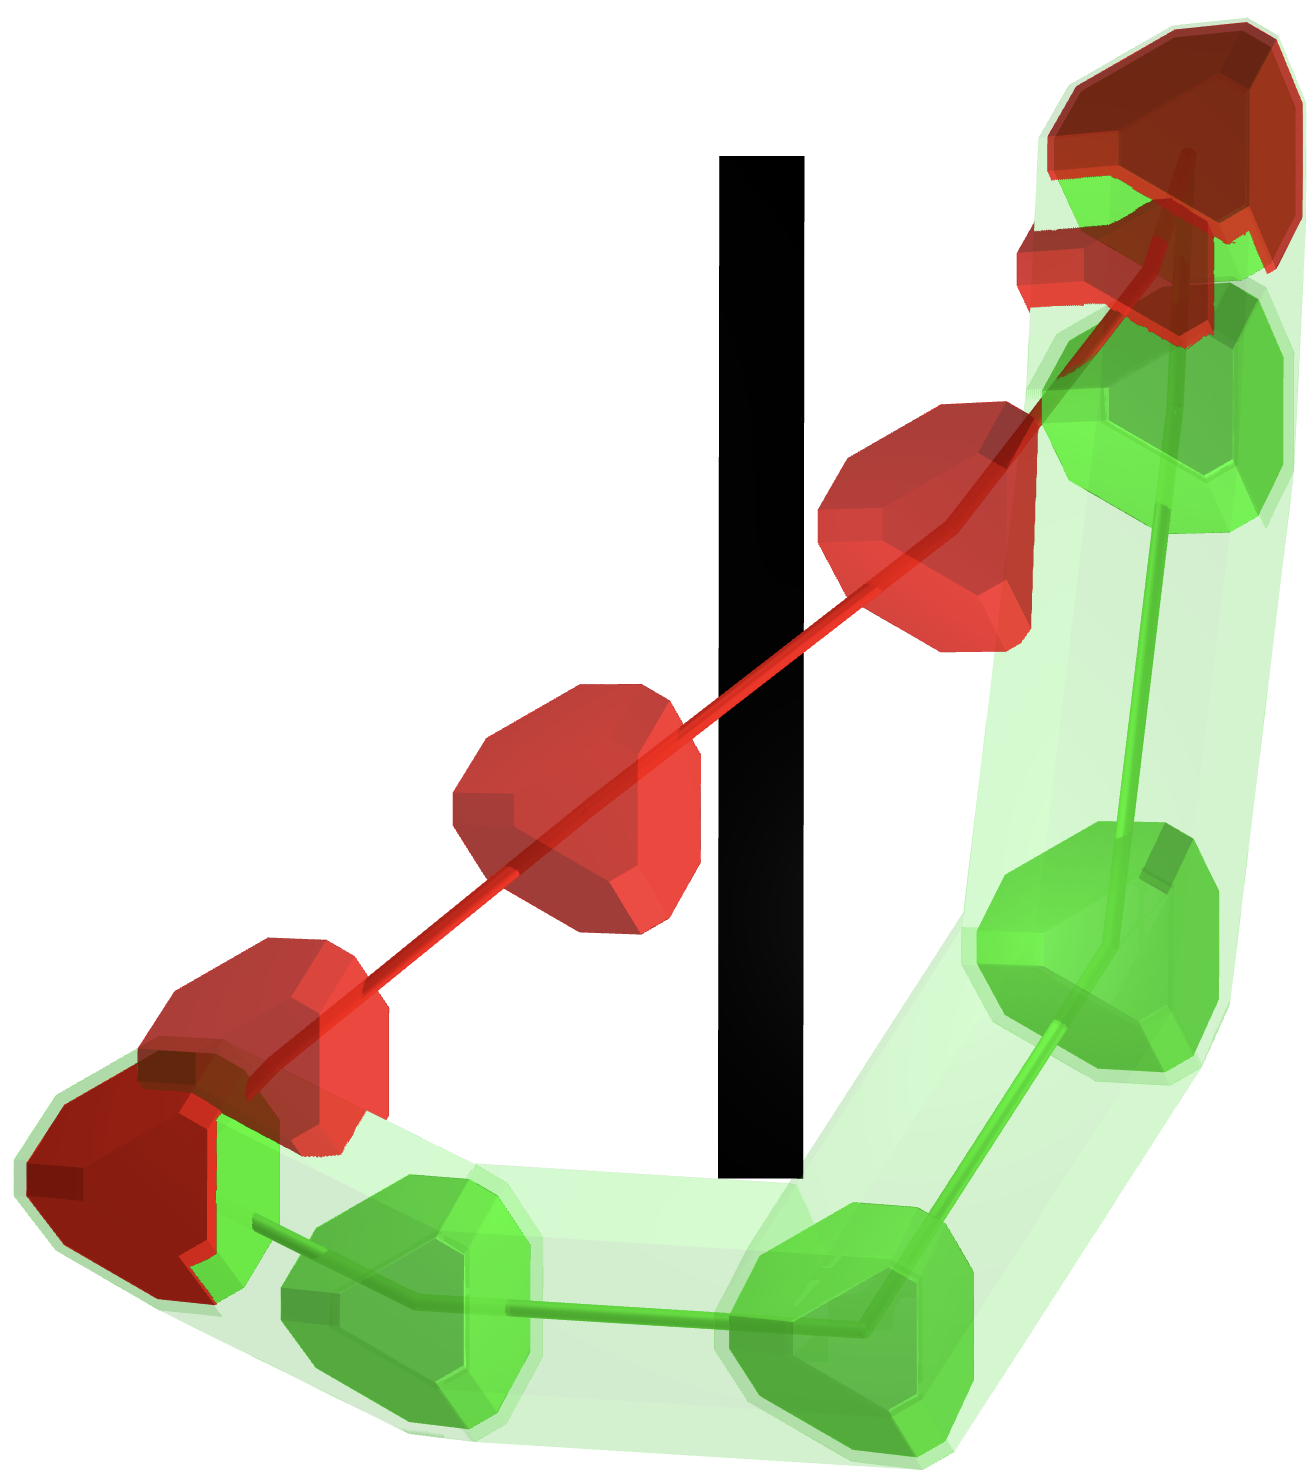
\includegraphics[width=2.4in]{figures/thru_wall/thru_wall_2.png}};
%     \node at (-3.615,3.085)[fill=red!90, text=white] {Discrete};
%     \node at (-3.4,2.4) [fill=green!90, text=black] {Continuous};
% \end{tikzpicture}
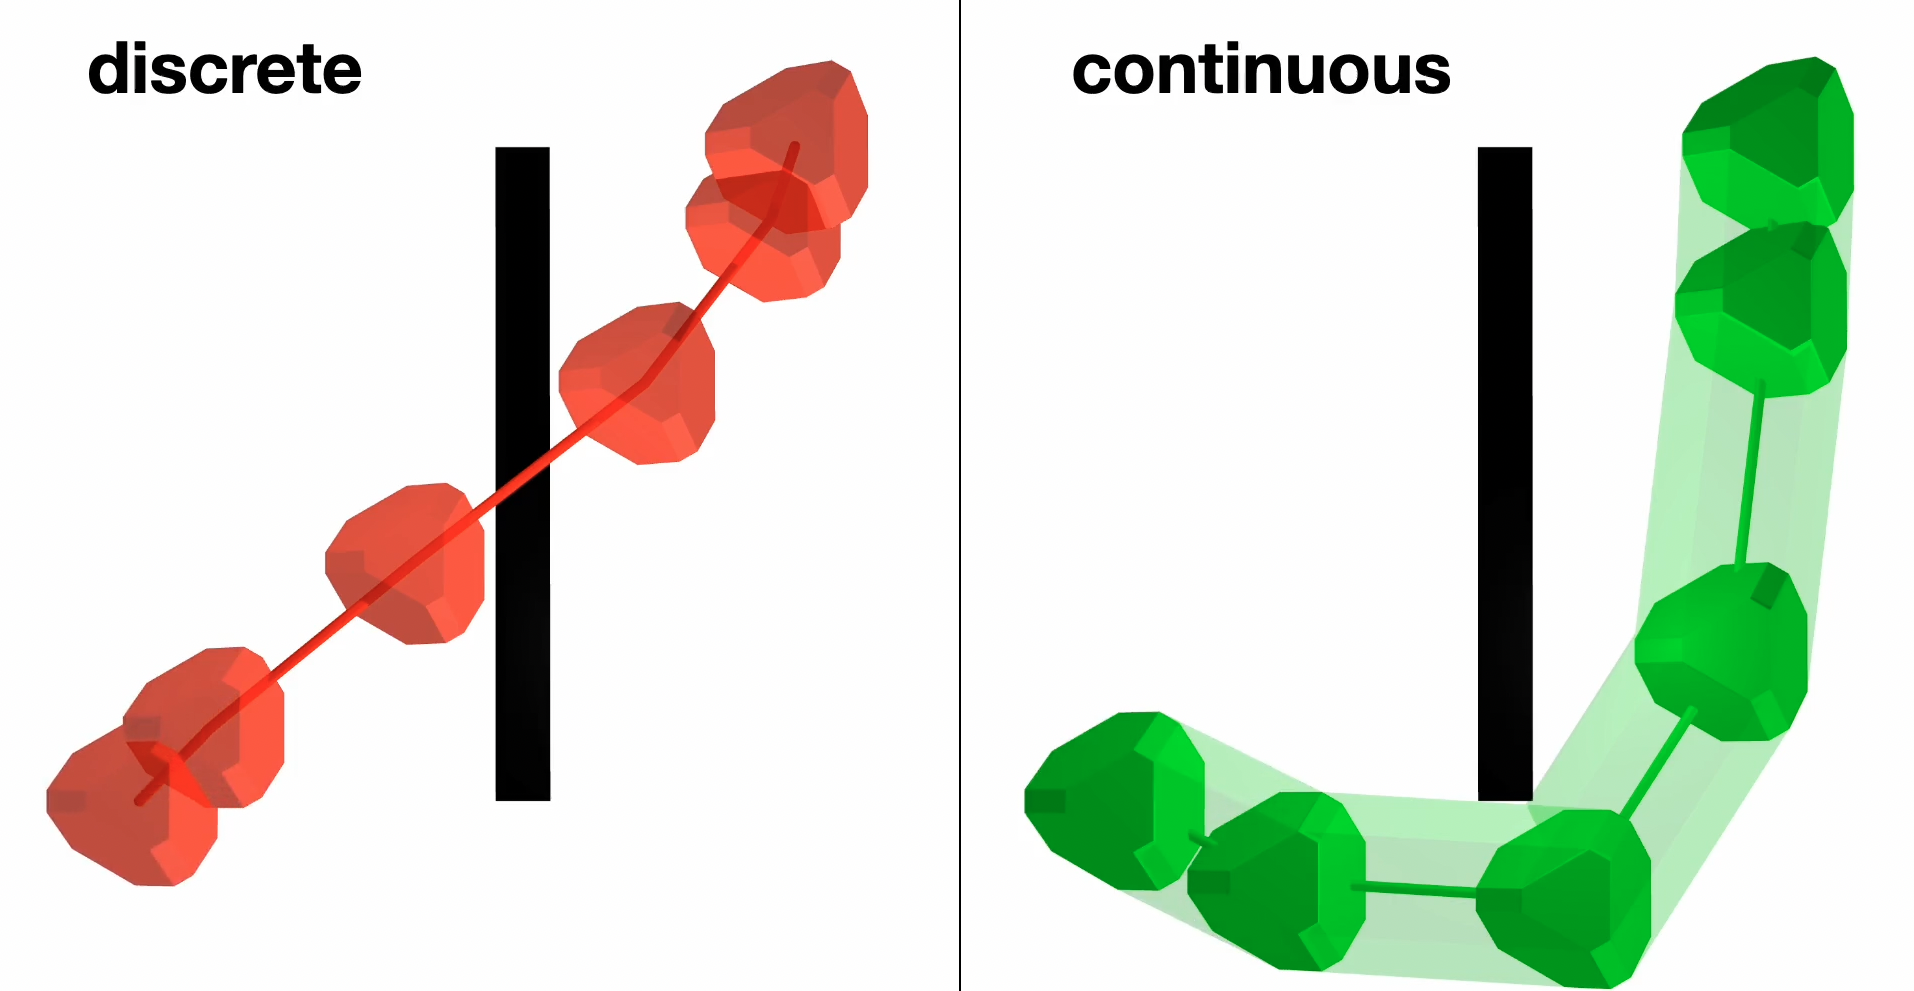
\includegraphics[width=.8\linewidth]{figures/thru_wall/thru_wall_3.png}
\caption{
Example trajectory optimization solutions for a polytope passing near a wall where collision avoidance constraints are specified with discrete collision detection (red) and the proposed continuous collision detection (green). In the discrete case, the solver only has to satisfy the collision avoidance constraints at each of the discrete knot points, allowing the polytope to ``speed'' through the wall while appearing collision-free to the solver. Using the proposed continuous collision detection, the solver is able to directly reason about collision that happen at and between the time steps to ensure that no collision exists.
}
\label{fig:thru_wall}
\end{figure}

To ensure that DCD is adequate for collision avoidance planning, a myriad of algorithmic enhancements have been proposed to combat these shortcomings. First, the time between discrete collision checks can be decreased, resulting in finer-grained collision checking at the expense of compute and problem complexity. Another common strategy is to add a collision margin that is conservative enough to combat any tunneling by making obstacles appear thicker than they are. In cuRobo~\cite{sundaralingam2023}, this collision margin is augmented with a penalty that effectively increases the margin when the robot is moving faster, thus discouraging any ``speeding through'' obstacles. In TrajOpt~\cite{schulman2013a}, collisions between pairs of convex objects at adjacent time steps are avoided by forming a convex hull for each object and checking these convex hulls for any intersections. This approach successfully captures continuous collisions but is a potentially limiting over approximation of the collision environment since the objects are not actually encompassing the convex hulls for the duration of the time step. 

Based on the complexity of the primitive, there are many available methods for DCD that each carry their own tradeoffs. For simple sphere-capsule-box interactions, analytical collision information can be solved for in closed form \cite{ericson2004}. For generic convex shapes, iterative methods such as Gilbert-Johnson-Keerthi (GJK) \cite{gilbert1988, cameron1997} and Minkowski Portal Refinement (MPR) \cite{snethen2008,newth2013} are used. Both GJK and MPR only return useful collision information when objects are not in contact; as soon as penetration occurs, the Expanding Polytope Algorithm (EPA) \cite{vandenbergen2001} must be used to determine a penetration depth. Highly mature implementations of these algorithms are available in the Flexible Collision Library (FCL) \cite{pan2012}, which many modern physics simulators rely on \cite{coumans2015,tedrake2019a,lee2018,todorov2012a}.  While these DCD algorithms are fast and reliable, they involve significant logic and branching, making them inherently nondifferentiable and challenging to put on a GPU. 
%
%

While DCD examines pairs of objects in static configurations, Continuous Collision Detection (CCD) reasons about objects as they move between sequential configurations. CCD computes the same information that DCD does, but in addition, also calculates the time of impact, indicating when a collision takes place between two configurations. This new information comes at an expense, as CCD is significantly more difficult and limited in the primitives it can handle compared to DCD. For simple sphere-capsule-box primitives, a mix of analytical and iterative methods are available for computing the time of impact~\cite{ericson2004}. In \cite{vandenbergen2004}, a GJK-based ray-casting method was proposed to compute the continuous collision information between a moving convex object and a static configuration-space obstacle. A method for direct handling of moving nonconvex meshes was introduced in \cite{zhang2006}, and was updated to include angular motion in \cite{coumans}. While these existing CCD methods are readily available, they suffer from the same branching and nondifferentiability issues as DCD methods.

This work focuses on convex-convex CCD as it relates to gradient-based motion planning, where cost and constraint functions are required to be differentiable. There has been growing interest in differentiable DCD with sampling-based methods \cite{montaut2022a}, and differentiable optimization-based methods \cite{tracy2023b,zimmermann2022,tracy2022}.  The work proposed in this paper serves more closely as a continuous follow-on to the differentiable DCD solution introduced in \cite{tracy2023b}, where a framework for computing smooth gradients through collision detection was enabled by scale-based collision detection and differentiable convex optimization. 

We introduce a true CCD routine for pairs of arbitrary convex sets that is fully differentiable with respect to each configuration. By solving for collision information with a geometric scale factor, the collision check reduces to a small convex optimization problem that is guaranteed to be globally solvable, bounded, and feasible for any configuration of the objects.  The solution of this optimization problem is then used to form smooth gradients of the collision information with respect to any problem parameters with very limited computational expense (significantly less than solving the problem). Together, this enables gradient-based motion planners to solve for collision-free trajectories with a coarse and efficient discretization of the trajectories.

Our specific contributions in this paper are the following:
\begin{itemize}
    \item An optimization-based continuous collision-detection method between pairs of moving convex sets without any branching or degenerate cases 
    \item A fast and efficient method for differentiating the method in automatic-differentiation frameworks
    \item A convex interior-point algorithm for solving the collision problem that can be arbitrarily parallelized on a GPUs or TPUs for problems with varying numbers of constraints
\end{itemize}

This paper proceeds by providing background information in Section \ref{sec:cdcol:background}, introducing our CCD algorithm in Section \ref{sec:cdcol:cdcol}, detailing a parallelizable convex solver in Section \ref{sec:cdcol:qp_solver}, examples of these methods used for collision avoidance motion planning in Section \ref{sec:cdcol:examples}, and our concluding remarks in Section \ref{sec:cdcol:conclusion}.
%
%
% \begin{figure}[t!]
%     \centering
%     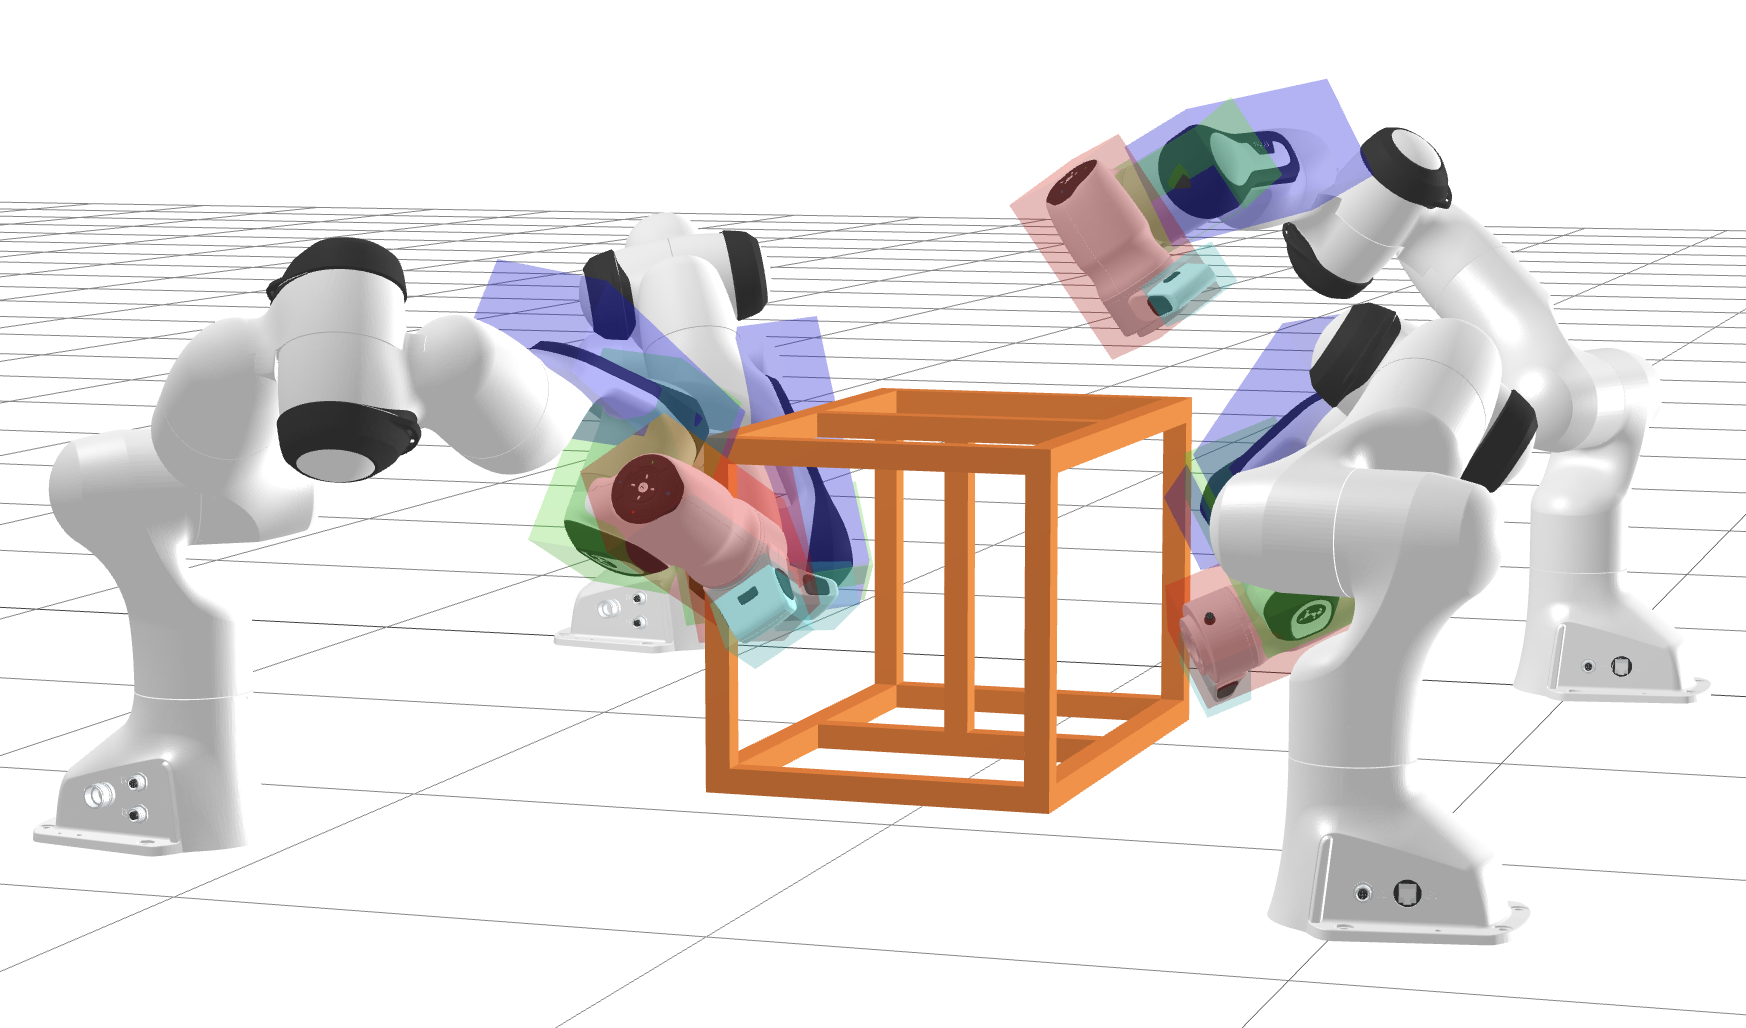
\includegraphics[width=.47\textwidth]{figures/ballet/ballet1.png}
%     \caption{A multi-robot assembly task where four robotic arms interact with a structure in a common workspace. The proposed continuous collision detection is used to certify trajectories as collision-free and is fully differentiable with respect to the configurations of the robots.}
%     \label{fig:growth}
% \end{figure}
%
%
\section{Background}\label{sec:cdcol:background}
%
%
%
%
The continuous collision-detection algorithm introduced in this paper involves forming, solving, and differentiating a convex optimization problem. In this section, the necessary background to understand this formulation is presented.

%
%
\subsection{Perspective Operators} \label{sec:cdcol:perspective}
% %
% %
% \begin{figure}[]
%     \centering
%     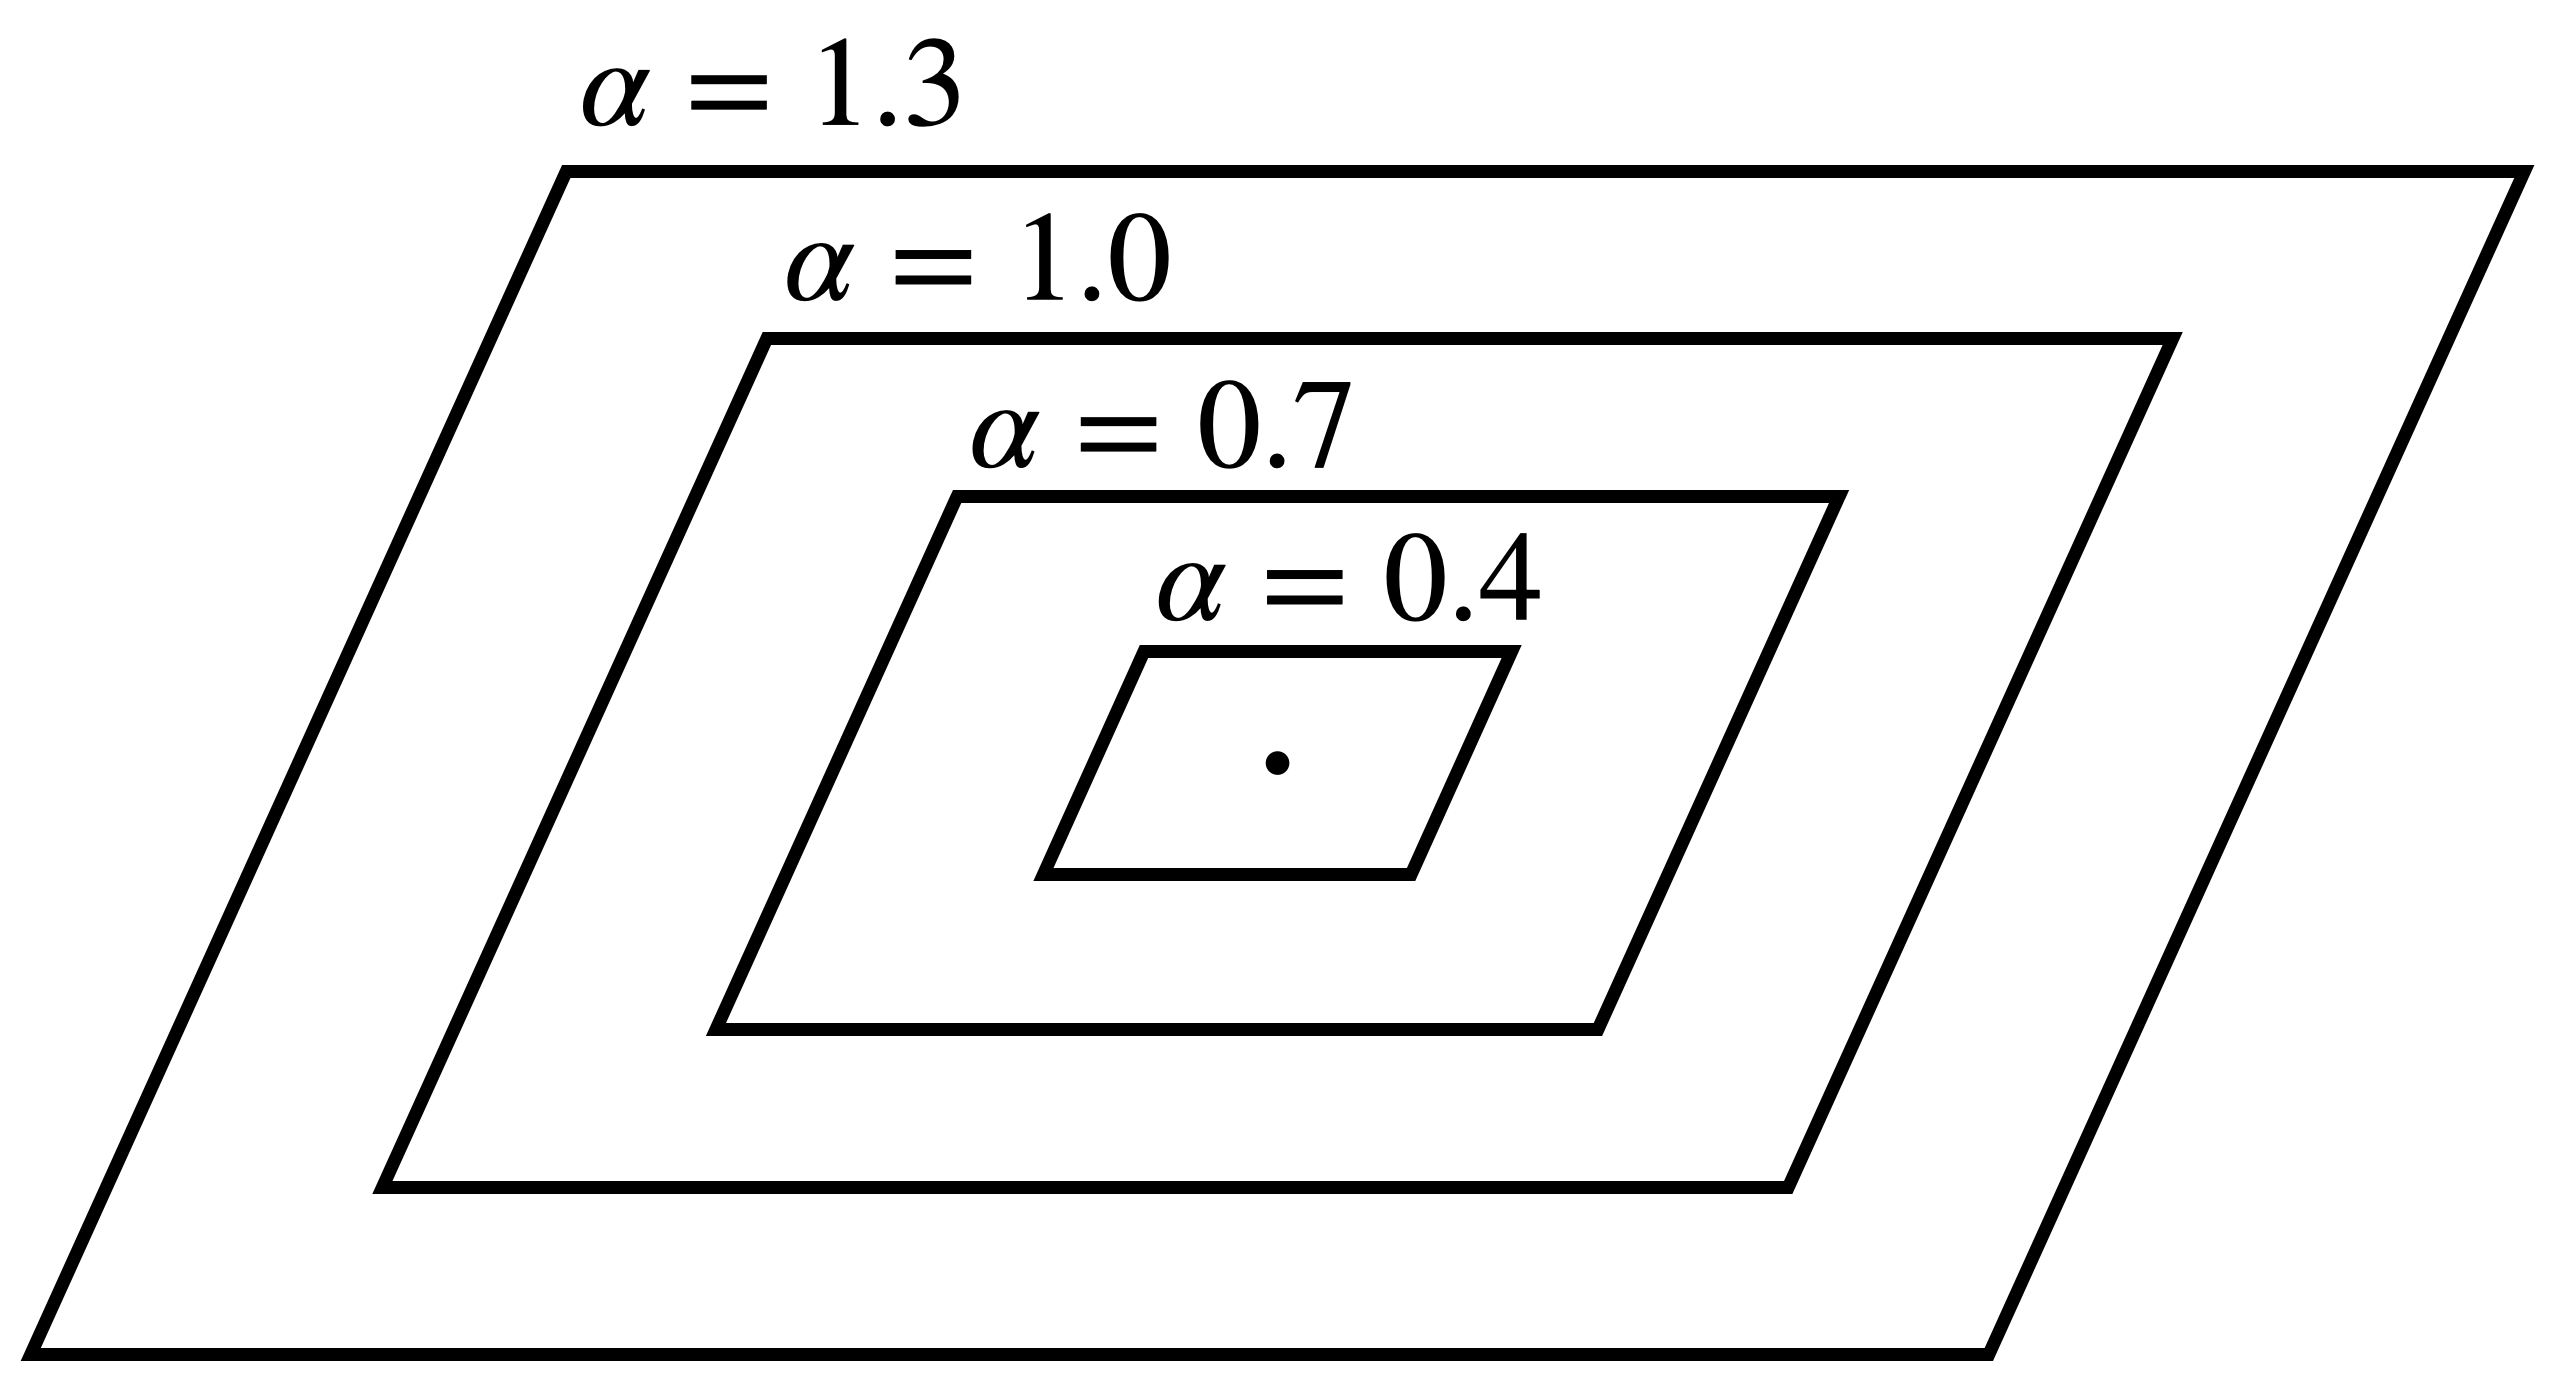
\includegraphics[width=.4\textwidth]{figures/growth/growth.png}
%     \caption{Demonstration of the scaling factor $\alpha$ as applied to a convex set. The original set, shown when $\alpha = 1$, is uniformly scaled down for $\alpha < 1$ and and up for $\alpha > 1$. As $\alpha \rightarrow 0$ the set becomes just a single point. This scaling idea is formalized as a perspective operator, where an arbitrary convex set can be scaled up and down in this fashion.}
%     \label{fig:growth}
% \end{figure}
% %
% %
In order to simplify the notation around scale-based collision detection, the idea of a perspective operator for a convex set is introduced. For collision purposes, each rigid body in a robot is decomposed into a collection of convex sets \cite{schulman2013a}.
Given a closed convex set $\mathcal{X} \subseteq \mathbf{R}^N$, a perspective operator is used to map this $n$-dimensional set to a cone in $n+1$ dimensions \cite{marcucci2023, marcucci, rockafellar1997, hiriart-urruty1993}.
The new dimension comes from a scale factor $\alpha \in \mathbf{R}_+$ that geometrically scales up the set when $\alpha > 1$ and scales down the set when $\alpha \leq 1$ until it is just a point at $\alpha = 0$. 
% This scaling and its effect on a convex set are demonstrated in Fig. \ref{fig:growth}. 

For practical purposes, the simplest way to exploit the perspective operator is to define the original convex set in standard conic form, $\mathcal{X} = \{x : Ax + b \in \mathcal{K}\}$, where $x \in \R{3}$ is a point in some world frame $\mathbb{W}$, and $\mathcal{K}$ is a proper convex cone \cite{boyd2004, lobo1998}. Common convex sets such as polytopes, cylinders, cones, capsules, and ellipsoids, can easily be represented in this form \cite{tracy2023b}. From here, the perspective operator defines a new scaled convex set $\bar{\mathcal{X}}$ as the following:
%
\begin{align}
    \bar{\mathcal{X}} &= \{(x, \alpha) : \alpha \geq 0, Ax + \alpha b \in \mathcal{K}\}.
\end{align}
%
For example, for a polytope described by $Bx + c \geq 0$ (where the cone $\mathcal{K}$ is the nonnegative orthant $\mathbf{R}_+$), the scaled polytope becomes $Bx + \alpha c \geq 0$.

It is often most convenient to express a convex set with an attached body frame $\mathbb{B}$, with an origin $\mathbb{B}_0$. Instead of redefining the convex set every time it moves in the world frame, we can instead simply define it once in its own body frame and parameterize any SE(3) rigid transformation with translation $r = {}^\mathbb{W} r {}^{\mathbb{B}_0}_\mathbb{B} \in \R{3}$ and rotation $Q = {}^\mathbb{W} Q {}^\mathbb{B} \in \R{3 \times 3}$. This allows us to write a general constraint for a convex set given a specific position and attitude as:
%
\begin{align}
    A Q^T(x - r) + \alpha b &\in \mathcal{K}. \label{eq:se3_standard_form}
\end{align}
%
This method for defining scaled convex sets in a world frame enables a straightforward extension to optimization-based collision detection built on this scaling. 
%
%
\subsection{Scale-Based Collision Detection}\label{sec:cdcol:background_scale_based}
%
%
\begin{figure}
\centering
\begin{tabular}{p{.6cm}cc}
\toprule
   &
  initial configuration & scaled to collision 
  \\
  \midrule
  \begin{tabular}{l}
    \small with \\
    \small collision
  \end{tabular} &
  \begin{tabular}{l}
   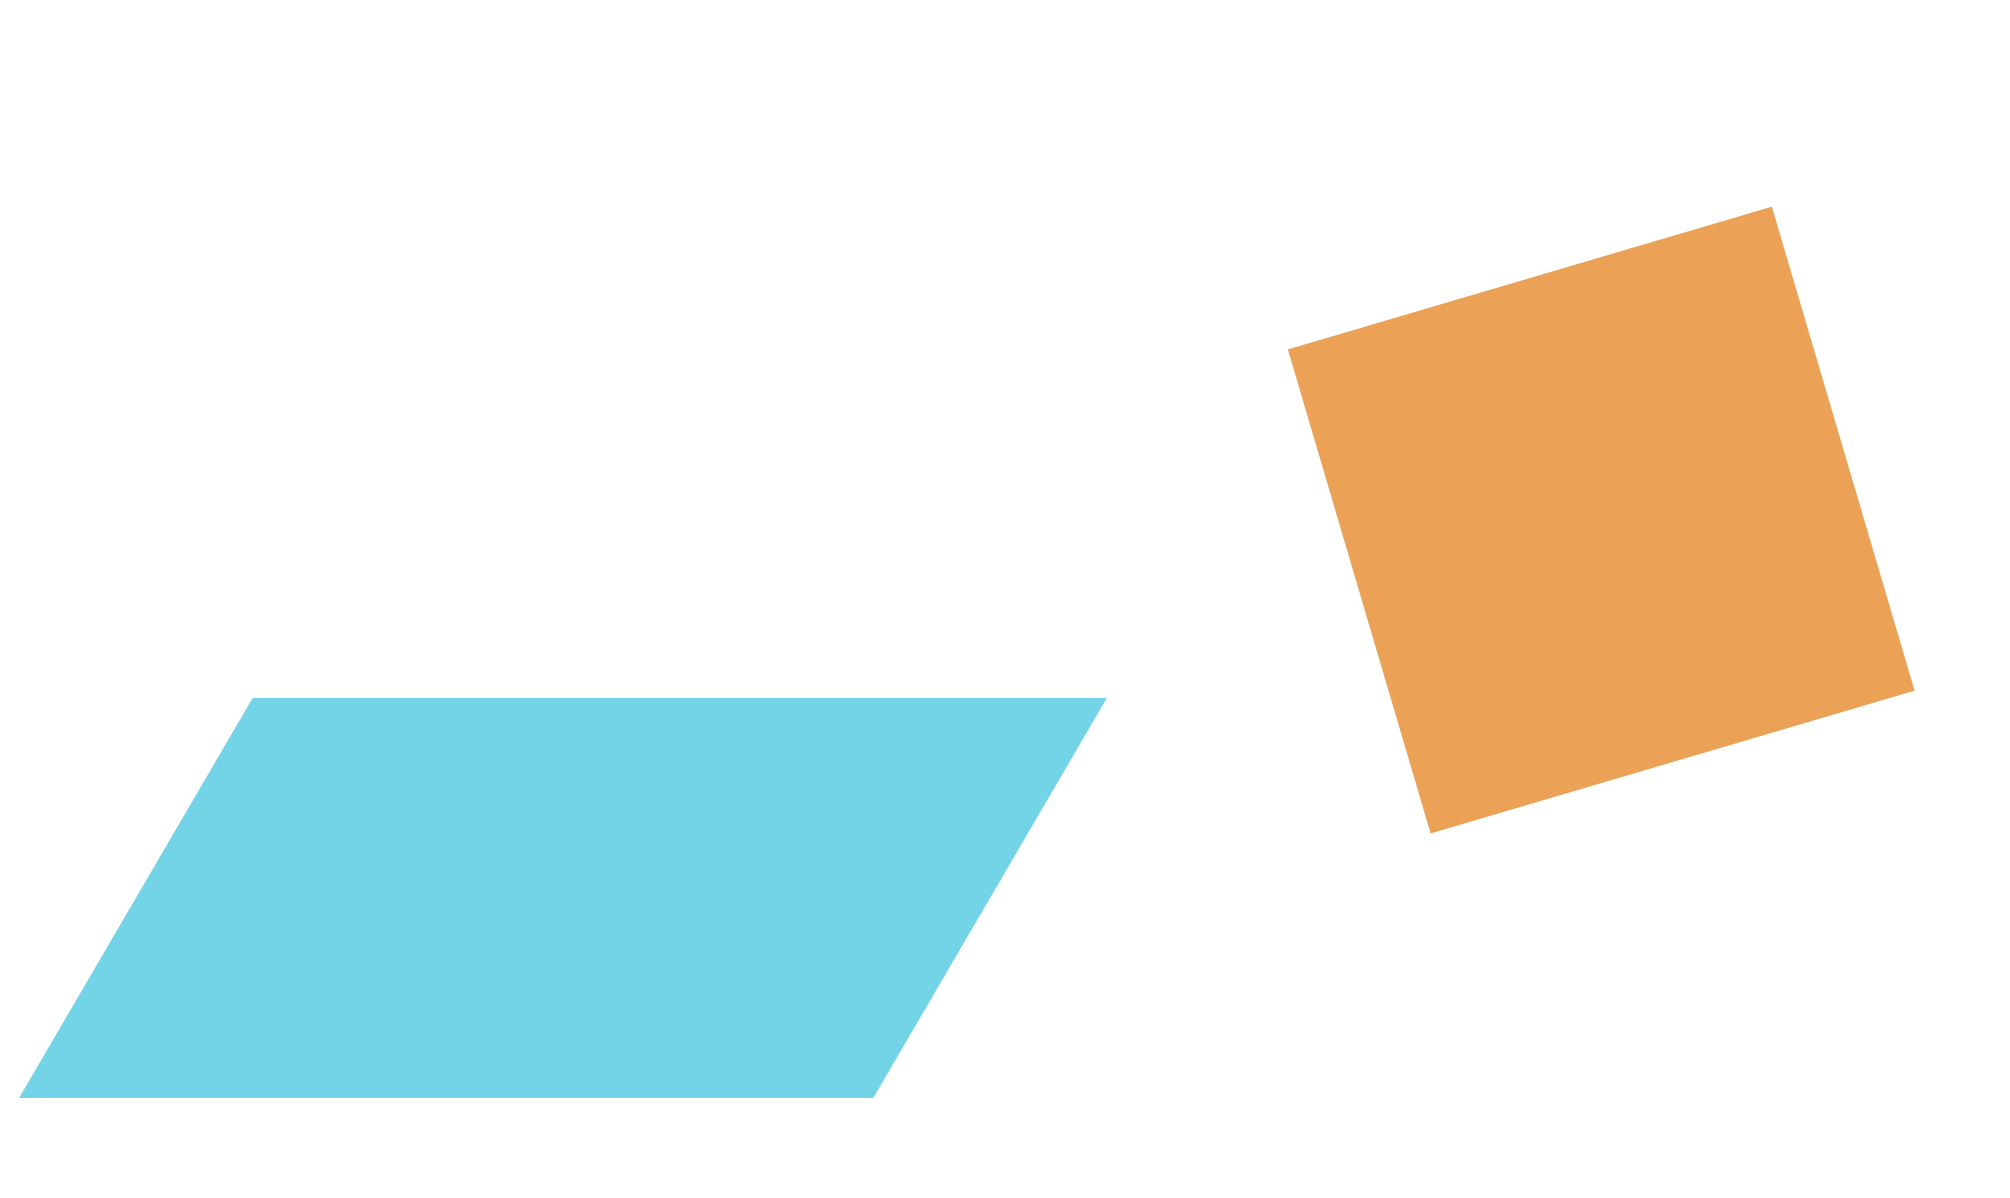
\includegraphics[height=1.5cm]{figures/four_panel/one.png}
  \end{tabular} & \begin{tabular}{l}
   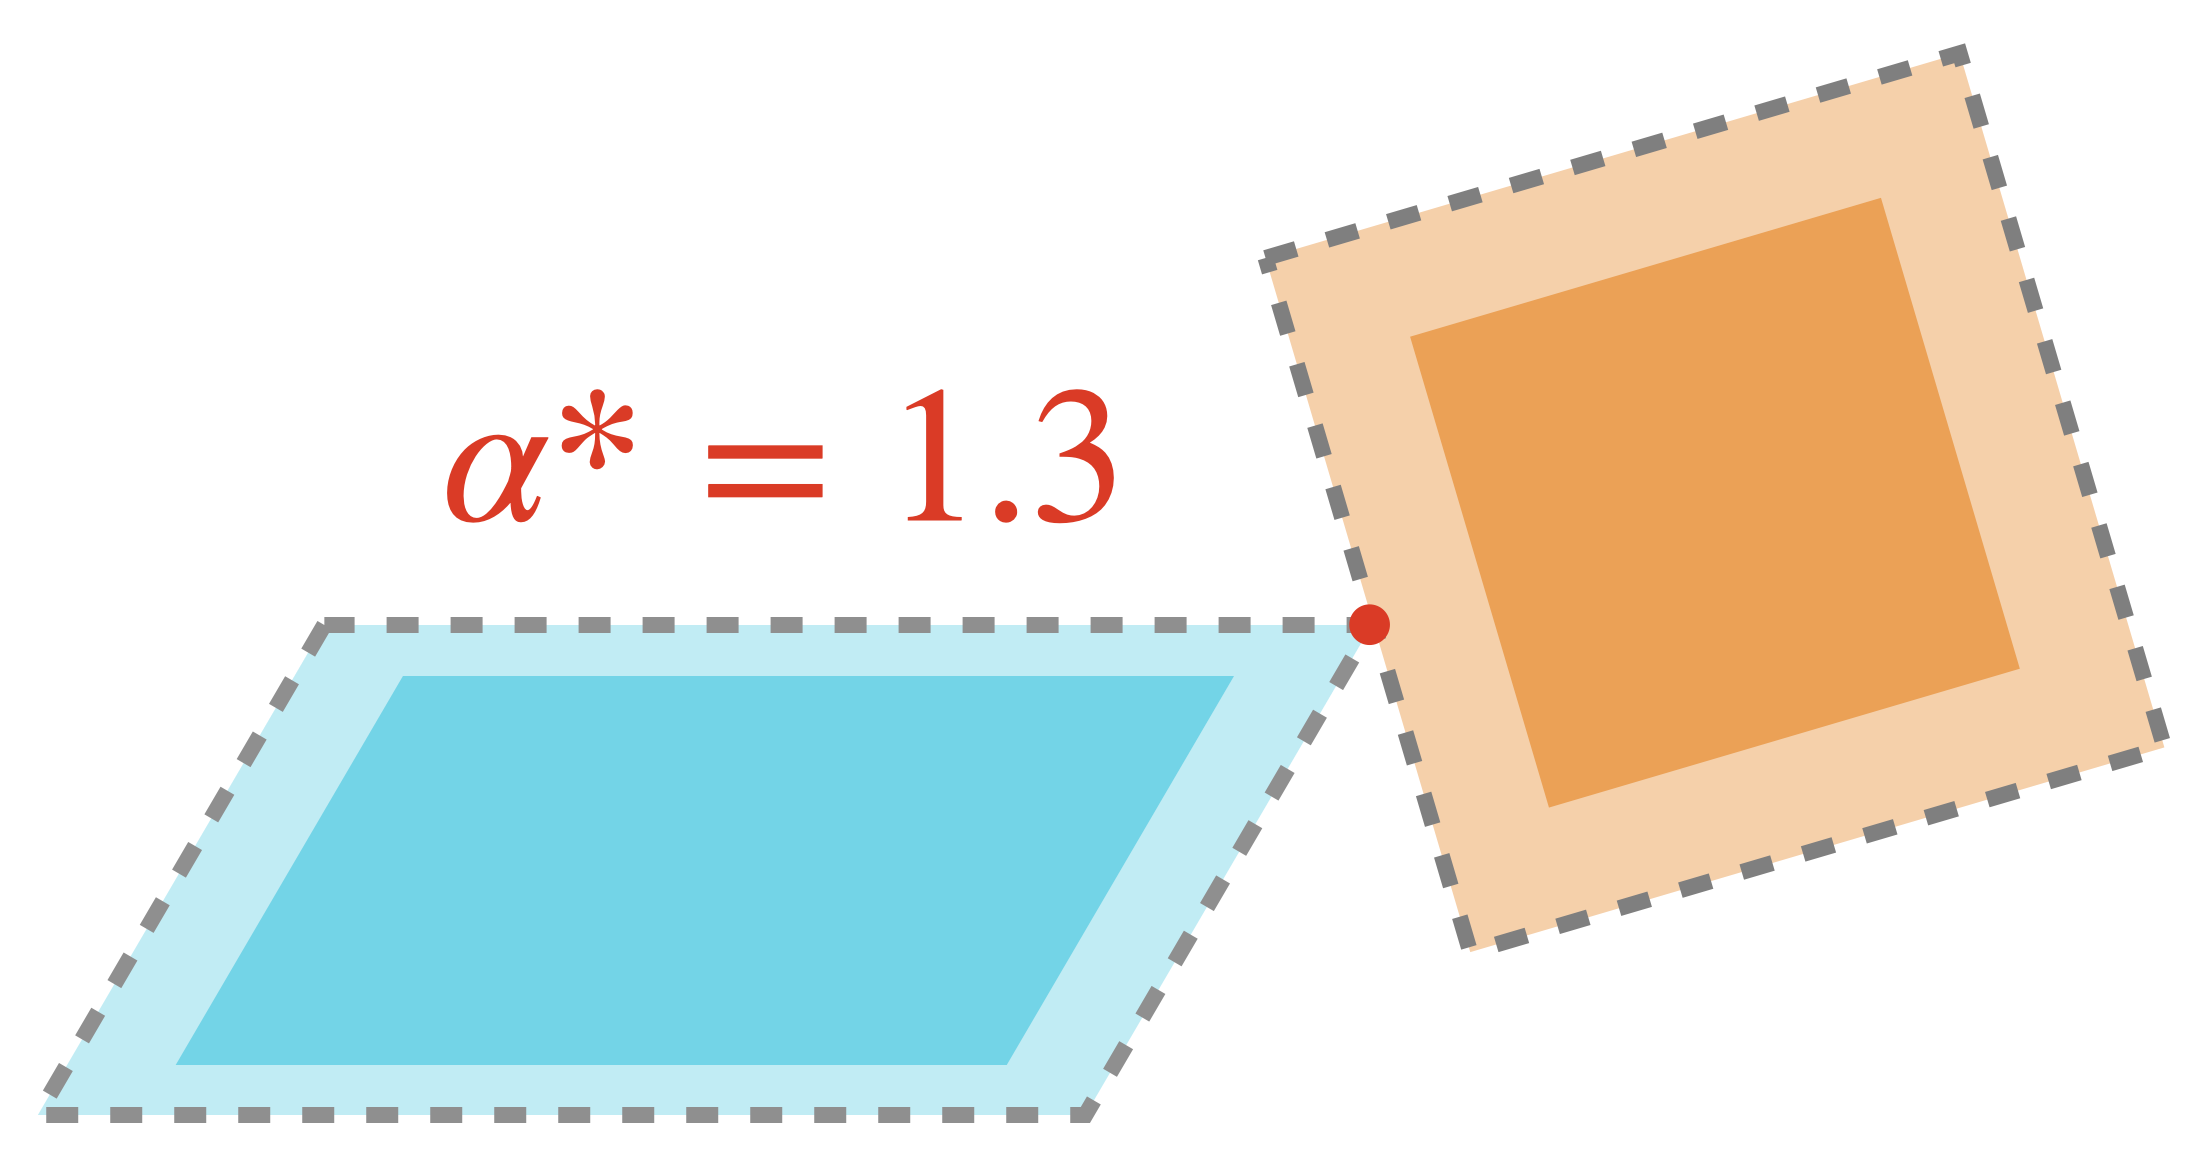
\includegraphics[height=1.5cm]{figures/four_panel/two.png}
  \end{tabular}\\
  % \hline
  \begin{tabular}{l}
    \small without \\
    \small collision
  \end{tabular} &
  \begin{tabular}{l}
    \begin{tabular}{l}
   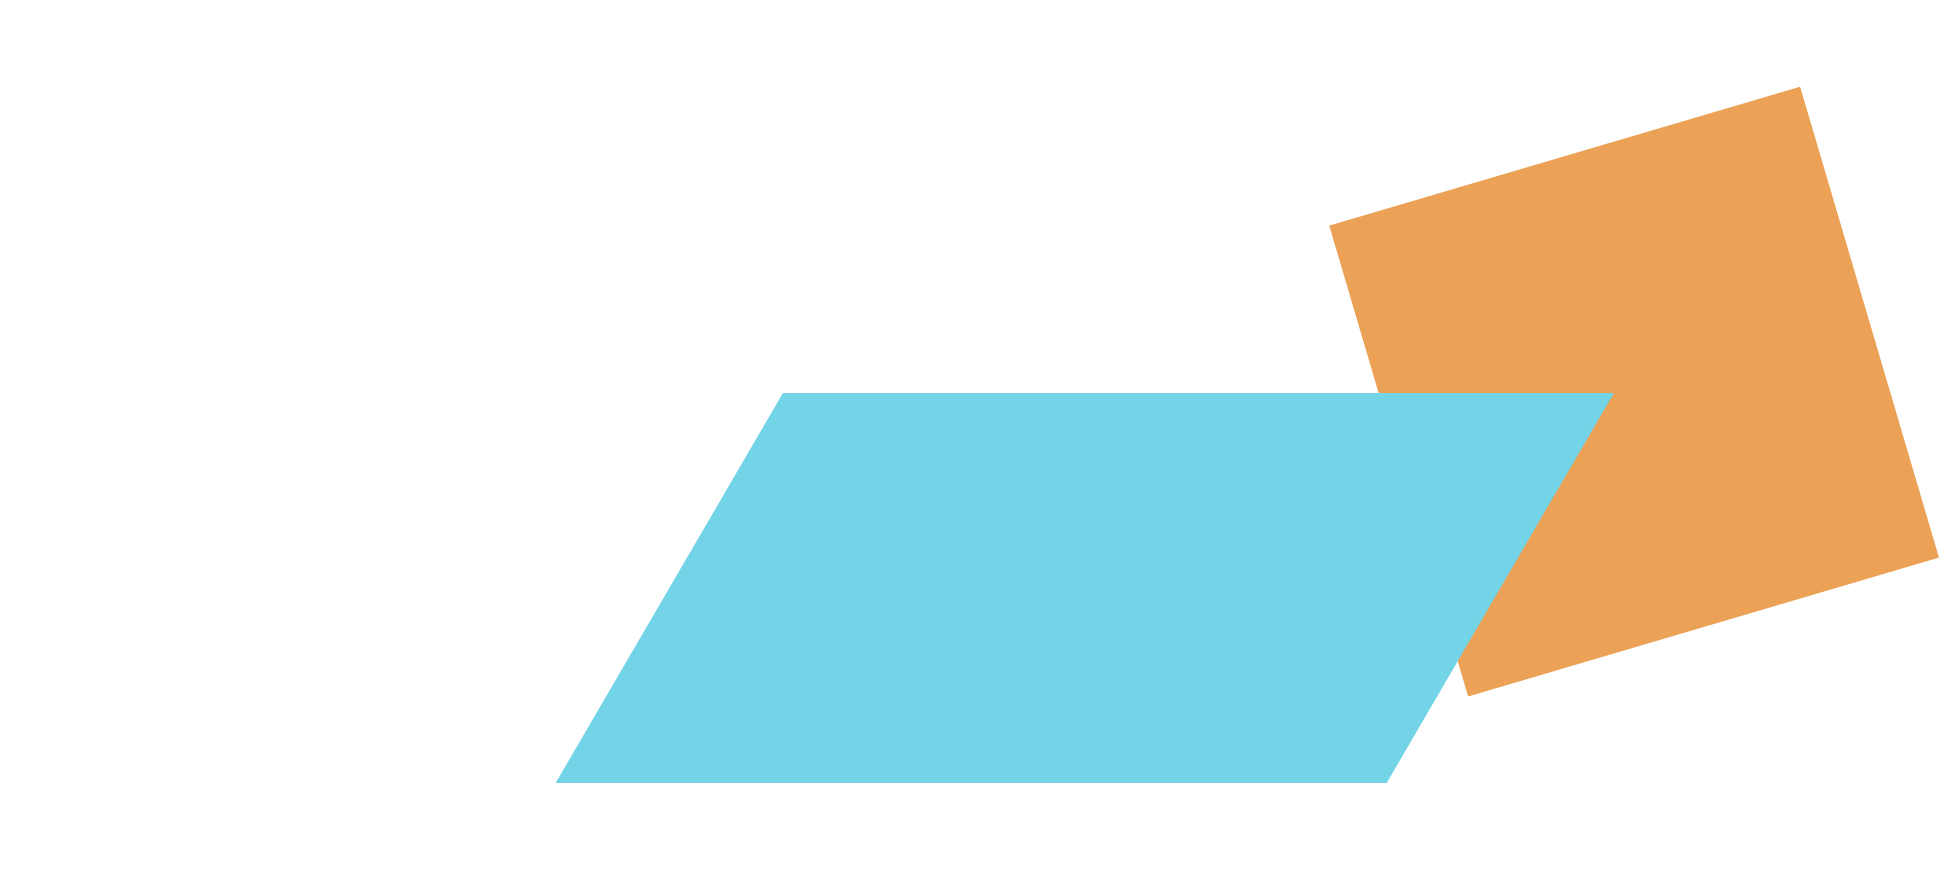
\includegraphics[height=1.1cm]{figures/four_panel/three.png}
  \end{tabular}
  \end{tabular} & \begin{tabular}{l}
   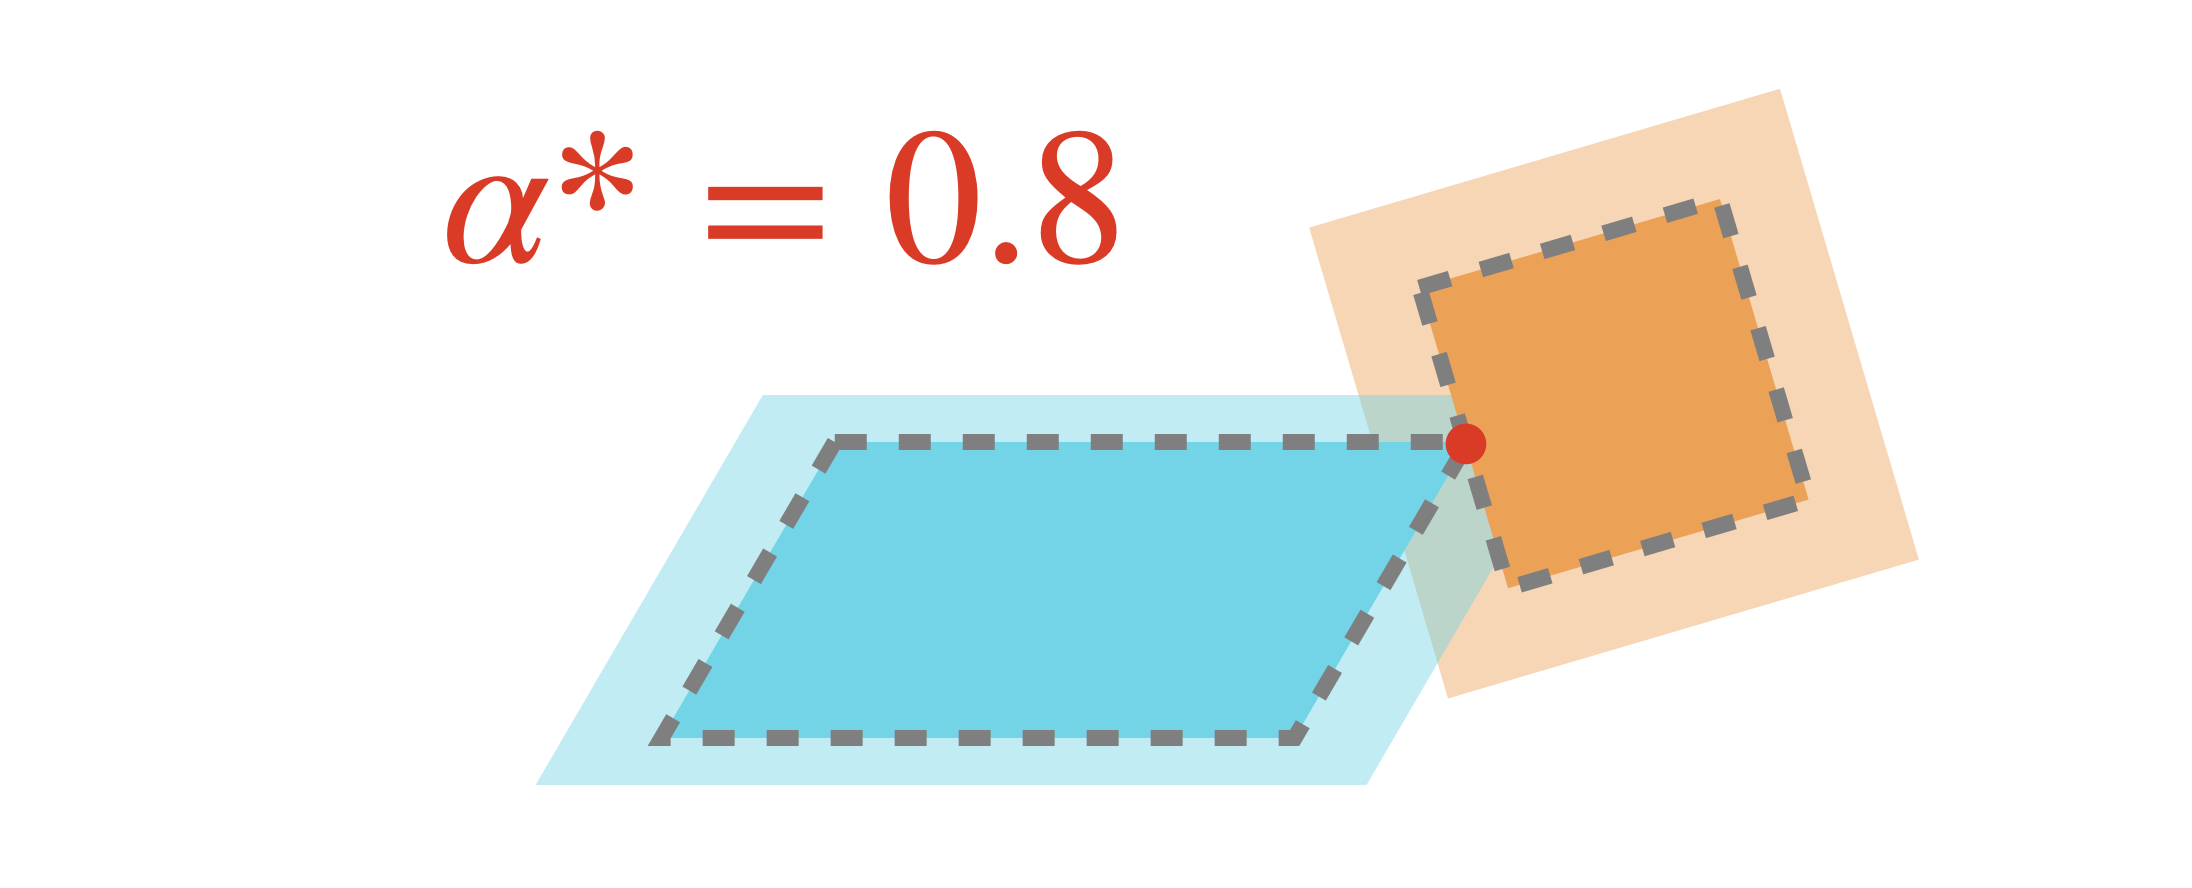
\includegraphics[height=1.1cm]{figures/four_panel/four.png} \end{tabular}\\
% \hline
\bottomrule
\end{tabular}
\caption{Scale-based collision detection for objects that are in and out of collision. In the upper row, the two objects are not in collision, so the minimum scaling that results in an intersection is able to ``grow'' the objects to $\alpha^* = 1.3$. In the bottom row, the two objects are already in collision, so the minimum uniform scaling shrinks the objects down to $\alpha^* = 0.8$.}
\end{figure}
%
%
Traditionally, collision detection between two convex sets is done by searching for the closest point between these two sets. If the closest points are not coincident, the objects are not in collision. This is the backing for the popular collision detection algorithms GJK~\cite{gilbert1988, cameron1997} and MPR~\cite{snethen2008,newth2013}, enabling fast and efficient collision detection between common convex primitives. The two main drawbacks of this approach come from nondifferentiability of these algorithms and the degenerate case when the two sets are in collision. In the latter case, GJK and MPR cannot return useful information and instead must default to an alternative algorithm such as EPA to establish a ``penetration depth.'' 

As shown in \cite{tracy2023b}, scale-based collision detection avoids both of these shortcomings by solving a different optimization problem. Instead of searching for the closest points between two fixed sets, the perspective operator is used to scale the two sets by a common $\alpha$ and solve for the minimum shared scaling that results in an intersection. 

With a point in the world frame $x \in \R{3}$ and two convex sets defined with \eqref{eq:se3_standard_form} as $A_iQ_i^T(x - r_i) + \alpha b_i \in \mathcal{K}$, the optimization problem that finds the minimum scaling $\alpha$ that results in an intersection between two scaled convex sets is:
%
\begin{mini}
{x, \alpha}{ \alpha}{\label{dcol2}}{}
% \addConstraint{A_1 Q_1^T(x - r_1) + \alpha b_1}{\in \mathcal{K}_1}{}
% \addConstraint{A_2 Q_2^T(x - r_2) + \alpha b_2}{\in \mathcal{K}_2}{}
\addConstraint{A_i Q_i^T(x - r_i) + \alpha b_i}{\in \mathcal{K}_i}{\quad i = 1, 2}
\addConstraint{\alpha}{\geq 0.}{}
\end{mini}
%
This is a convex optimization problem that is guaranteed to be both feasible and bounded. In the event that the two convex sets are in collision, the sets are scaled down to $\alpha < 1$ to the smallest possible scale factor that has an intersection. If the two sets are not in collision, they are scaled up to $\alpha > 1$ until an intersection is reached. In both cases, the fundamental algorithm remains unchanged, as the optimization formulation in ~\eqref{dcol2} handles both cases. Furthermore, there are no degenerate cases based on the geometry or configurations of the sets, since there always exists a minimum scaling for an intersection, even when the intersection is another set (a line or a plane). 
%
%
\subsection{Differentiable Optimization}
%
%
Collision detection as a solution to an optimization problem in \eqref{dcol2} makes taking derivatives with automatic differentiation tools challenging. Both forward and reverse-mode automatic differentiation are unable to accurately compute derivatives through an iterative numerical solver \cite{amos2017}. To avoid this, differentiable optimization tools are used to compute these derivatives in a fast and accurate way without propagating derivatives through iterative schemes.

Given a generic optimization problem in the following form:
%
\begin{mini}
{y}{ f_\theta(y)}{\label{generic_opt}}{}
\addConstraint{c_\theta(y)}{\in \mathcal{K},}{}
\end{mini}
%
with the cost and constraints as functions of some problem parameters $\theta$, a dual variable $\lambda \in \R{m}$ is used to enforce the constraint in the following Lagrangian:
%
\begin{align}
    \mathcal{L}_\theta(y, \lambda) &= f_\theta(y) + \lambda^Tc_\theta(y).
\end{align}
%
Using this, the KKT conditions necessary for optimality are,
%
\begin{align}
    \nabla_y f_\theta(y) + \bigg[ \frac{\partial c}{\partial y} \bigg]^T\lambda  &= 0 \label{kkt:1} \\ 
    c_\theta(y) &\in \mathcal{K}\label{kkt:2} \\ 
    \lambda &\in \mathcal{K}^* \label{kkt:3}\\ 
    c_\theta(y) \circ \lambda &= 0,\label{kkt:4}
\end{align}
%
where $\mathcal{K}$ is a proper cone and $\mathcal{K}^*$ and $\circ$ are the corresponding dual cone and cone product, respectively \cite{vandenberghe}. Any primal-dual values $(y, \lambda)$ that satisfy equations \eqref{kkt:1}-\eqref{kkt:4} are a locally optimal solution to \ref{generic_opt}.

By viewing equations \eqref{kkt:1} and \eqref{kkt:4} as the following implicit function of $w = (y, \lambda)$,
%
\begin{align}
    g_\theta(w) &= \begin{bmatrix}
        \nabla_y f_\theta(y) + \big[ \frac{\partial c}{\partial y} \big]^T\lambda \\ 
         c_\theta(y) \circ \lambda
    \end{bmatrix},
\end{align}
%
an approximate primal-dual solution $w^* = (y^*, \lambda^*)$ is an equilibrium point where $g_\theta(w^*) \approx 0$. At this equilibrium, the implicit function theorem can be used to calculate the Jacobian of the primal-dual solution with respect to the to the problem parameters \cite{howell2022}:
%
\begin{align}
    \frac{\partial y}{\partial \theta} = - \bigg( \frac{\partial g}{\partial y} \bigg)^{-1}\frac{\partial g}{\partial \theta}. \label{eq:ift2}
\end{align}
%
Practically, this works by solving the problem with a standard numerical solver, after which the approximate solution is used with the implicit function theorem to provide the necessary derivatives.

Alternatively, if the only derivative we need is that of the optimal objective value $f(x^*)$ with respect to the problem parameters, an even simpler approach can be used: At a primal-dual solution, the gradient of the objective value with respect to the problem parameters is simply the gradient of the Lagrangian with respect to these same parameters \cite{castillo2006},
%
\begin{align}
    \nabla_\theta f_\theta(y^*)= \nabla_\theta \mathcal{L}_\theta(y^*, \lambda^*), \label{eq:lag_grad}
\end{align}
%
allowing us to calculate the derivative we need without forming or solving a linear system.

These differentiable optimization methods are used to convert the always-feasible convex optimization problem in \eqref{dcol2} into a fully differentiable algorithm, as shown in \cite{tracy2023b}. The optimal objective value ($\alpha$) or the primal and dual variables can be differentiated with respect to both the configurations of the objects and the geometry of the objects themselves. In \cite{tracy2023b} this was used in trajectory optimization to solve for collision-free trajectories simply by enforcing $\alpha > 1$ as a differentiable constraint in a motion planner.
%
%
%
%
\section{Continuous Collision Detection}\label{sec:cdcol:cdcol}
%
%
%
%
\begin{figure*}[t!]
    \centering
    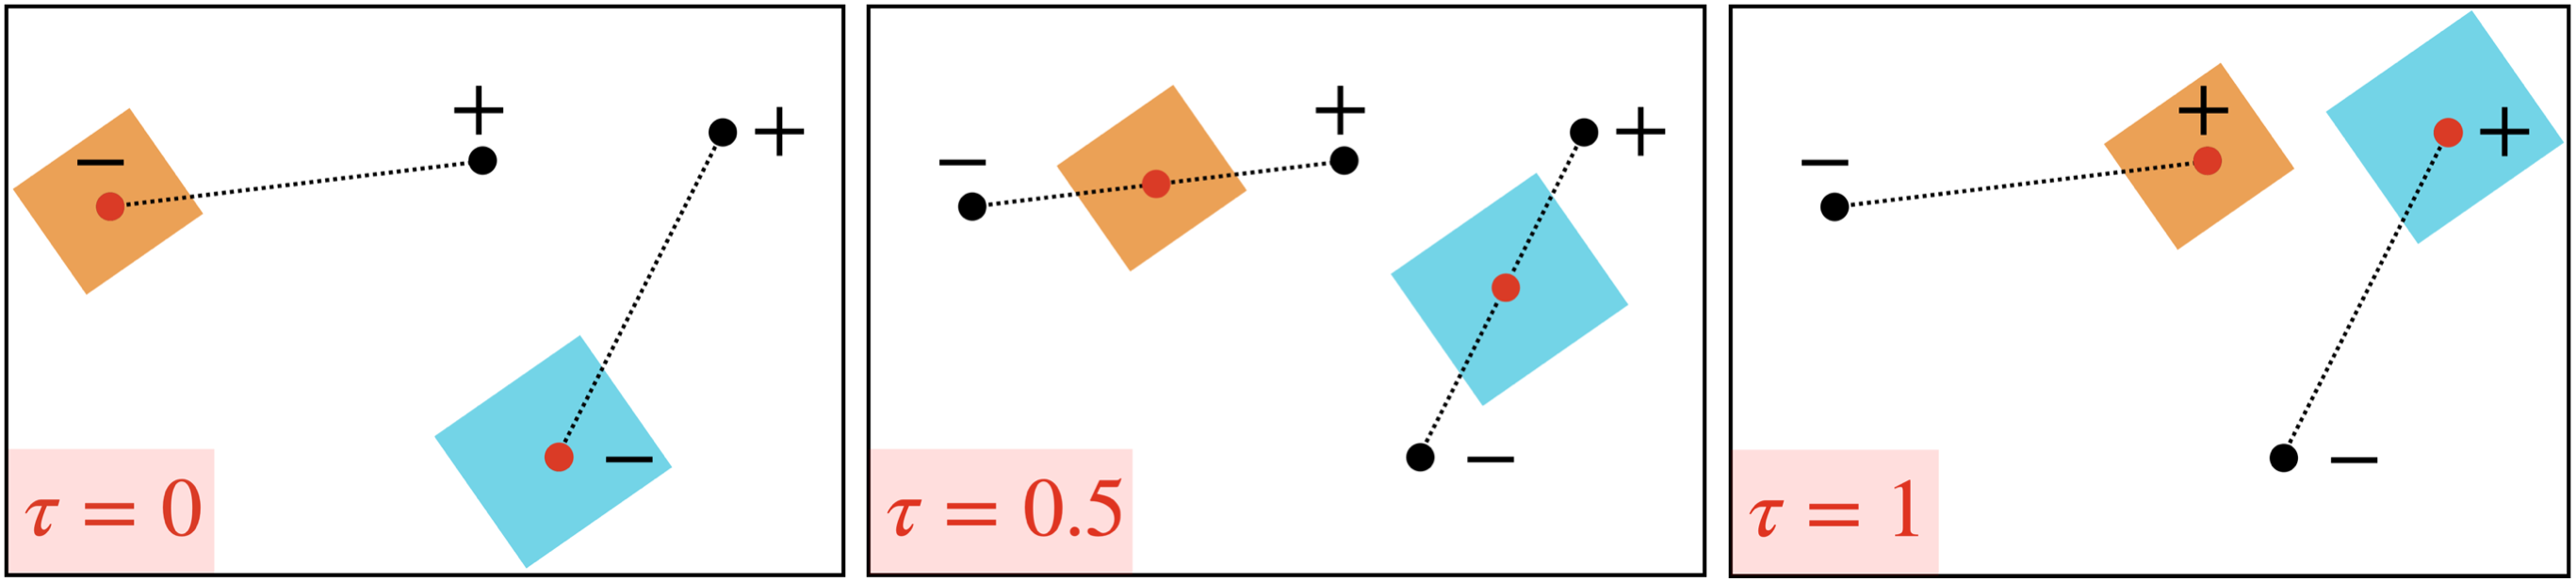
\includegraphics[width=.8\textwidth]{figures/tau/third.png}
    \caption{Graphical description of how the $\tau \in [0, 1]$ parameter linearly interpolates the origin of the objects from their initial positions at $r_i^{(-)}$ at $\tau = 0$, to $r_i^{(+)}$ at $\tau = 1$. Discrete collision detection can only check objects for collisions at $\tau = 0$ and $\tau = 1$, while the proposed continuous collision detection method can determine whether there is a collision as each object moves between the two positions. It is important to note that this sweeping motion is \textit{not} simply checking if two convex hulls are in collision, but rather checks for contact as both objects move simultaneously on the path.}
    \label{fig:sweep_tau}
\end{figure*}
%
With the necessary background on perspective operators, scale-based collision detection, and differentiable optimization, the novel CCD algorithm can now be introduced that checks for collisions between two convex sets as they move between configurations. 

The core assumption in this CCD framework is that the two objects move linearly between time steps with a fixed attitude. This motion can be seen in Fig. \ref{fig:sweep_tau}, where two shapes ``sweep'' between the time steps. Given the two convex sets with positions $r_i \in \R{3}$ and attitudes $Q_i \in \R{3 \times 3}$, as described in Section \ref{sec:cdcol:perspective}, we can introduce the notation for time. Positions and attitudes from the first time step will be denoted with
$\Box^{(-)}$, and those from the second time step with $\Box^{(+)}$. A new normalized time parameter $\tau \in [0,1]$ is introduced where $\tau=0$ denotes the first time step and $\tau = 1$ denotes the second. Together, we can express this notation as $r_i(\tau=0) = r_i^{(-)}$, and $r_i(\tau=1) = r_i^{(+)}$. A line segment between these two positions can be calculated with the following,
%
\begin{align}
    r_i(\tau) = \tau r_i^{(-)} + (1 - \tau)r_i^{(+)},
\end{align}
%
where we simply linearly interpolate from the position at one time step to the position at the next with a constant linear velocity.  The attitudes between the time steps are simply averaged as $Q_i$, which is straightforward depending on the parameterization of the attitude~\cite{markley2014, markley2007}. Now, a scale-based collision-detection problem, similar to \eqref{dcol2}, is introduced as follows,
%
\begin{mini}
{x, \alpha, \tau}{ \alpha}{\label{cdcol}}{}
\addConstraint{A_i Q_i^T(x - \tilde{r}_i) + \alpha b_i}{\in \mathcal{K}_i,}{ \quad i = 1,2}
\addConstraint{\tau r_i^{(-)} + (1 - \tau)r_i^{(+)}}{= \tilde{r}_i,}{\quad i = 1,2}
\addConstraint{0 \leq \tau }{\leq 1}{}
\addConstraint{\alpha}{\geq 0,}{}
\end{mini}
%
where we are searching for the minimum positive scale factor $\alpha$ such that an intersection exists between the two scaled convex sets as they sweep between the time steps.  Similar to \eqref{dcol2}, a collision exists if and only if $\alpha^* \leq 1$. This is a small convex optimization problem that is guaranteed to have a solution no matter the configuration of the objects. It makes no difference to the algorithm if the objects are in or out of collision for any amount of the sweep, or if they don't collide at all. The constraint $\alpha \geq 0$ is written here as a formality, since it is implicitly satisfied by the perspective operator.

Once this problem is formed and solved, the primal and dual variables can be used to calculate the gradients of the optimal $\alpha^*$ with respect to the poses or geometries of the objects using \eqref{eq:lag_grad}. If Jacobians of the primal or dual variables with respect to the problem parameters are needed, the implicit function theorem can be used to form these derivatives with \eqref{eq:ift2}. 

For numerical stability, it is often advantageous to add a very small regularization term to \eqref{cdcol},
%
\begin{align}
    J_{{reg}} &= \epsilon [\|x - r_{avg}\|_2^2 + (\alpha - 1)^2 + (\tau - 0.5)^2 ],
\end{align}
%
where $\epsilon << 1$ and $r_{avg} \in \R{3}$ is the average of the four positions (two objects at two time steps). This regularizer serves to guarantee that \eqref{cdcol} is \textit{strongly} convex, and can sometimes help the solver converge in fewer iterations \cite{boyd2004,nocedal2006}. With a small regularizer in the range $\epsilon \in [10^{-8}, 10^{-5}]$, the regularized optimal objective value does not differ meaningfully from $\alpha^*$.
%
%
% \subsection{Time of Collision Formulation}
% %
% %
% \todo{I may remove this section}
% If a collision has been identified with \eqref{cdcol}, it may be of interest when the Time of Collision (TOC) is. This can also be solved in an optimization-based way with a very similar formulation. Instead of minimizing the scaling that results in an intersection, we can fix $\alpha = 1$ and solve for the minimum $\tau$ that results in a collision:
% %
% \begin{mini}
% {x, \tau}{ \tau}{\label{toc}}{}
% \addConstraint{A_i Q_i^T(x - \tilde{r}_i) + b_i}{\in \mathcal{K}_i,}{ \quad i = 1,2}
% \addConstraint{\tau r_i^{(-)} + (1 - \tau)r_i^{(+)}}{= \tilde{r}_i,}{\quad i = 1,2}
% \addConstraint{0 \leq \tau }{\leq 1.}{}
% \end{mini}
% %
% This problem is again a small convex optimization problem that can be solved and differentiated quickly. Unlike \eqref{cdcol}, this problem will not have a feasible solution if there is no collision, so it should only be solved if \eqref{cdcol} has already identified a collision.
%
%
%
%
\section{Parallelizable QP Solver}\label{sec:cdcol:qp_solver}
%
%
%
%
In this section, a fast and efficient Primal-Dual Interior-Point (PDIP) solver will be described that is capable of running in parallel on accelerator units (GPU/TPU). Since the optimization problem in \eqref{cdcol} is small (5 primal variables), state-of-the-art PDIP methods can solve this problem quickly and reliably. We focus on polytopes as our convex primitive, as they are expressive and result in \eqref{cdcol} being a convex Quadratic Program (QP).  

Writing convex optimization solvers on a GPU has become significantly easier in recent years, with the advent of domain-specific languages like PyTorch \cite{paszke2019} and JAX \cite{bradbury2018}. High-level Python code can be compiled to run directly on GPUs/TPUs allowing for massively parallel computation with minimal implementation effort. 

The challenge in scaling up these computations for our proposed collision detection comes from the varying sizes of the convex sets in the scene. Since we are focusing on polytopes in this section, this translates to dealing with polytopes with different numbers of faces. In JAX, the best way to parallelize a computation is to call the same function over a list of equal sized arrays. In the case of polytopes with varying numbers of faces, this results in QPs with different numbers of constraints, violating our assumption of equal-sized arrays. 

In order to ensure that the arrays being parallelized over are of equal size, many algorithms simply choose the largest array in the set and pad all of the smaller arrays with zeros. In the case of constraints for a QP solver, this results in redundant constraints, violating the Linear Independence Constraint Qualification (LICQ) assumption that many solvers rely on to function properly \cite{nocedal2006, howell2022}. Violations of LICQ result in solvers failing due to rank-deficient linear systems caused by a nonuniquness of the dual variables. We propose a custom PDIP algorithm that solves the necessary linear systems with a block reduction that is capable of handling redundant constraints. 

The solver presented in Alg. \ref{pdip} handles convex QPs in the following form:
%
\begin{mini}
{x, s}{ \frac{1}{2}x^TPx + q^Tx}{\label{qp}}{}
\addConstraint{Gx + s}{= h}{}
\addConstraint{s}{\geq 0,}{}
\end{mini}
%
with a primal and slack variable $x \in \R{n}$ and $s \in \R{m}$ , a cost described with $P \in \mathbb{S}^n_+$ and $q \in \R{n}$, and an inequality constraint described with $G \in \R{m \times n}$ and $h \in \R{m}$.  The constraint is enforced with a dual variable $z \in \R{m}$, and the only requirement for the initialization of this solver is $(s, z) \geq 0$. An advanced initialization from \cite{mattingley2012} can also be used for added robustness.

To ensure that all the problem instances have the same number of constraints, the inequality constraint parameters $G$ and $h$ are padded with zeros. To avoid numerical problems in the solver, care is taken to use a binary mask vector $m \in \R{m}$ that identifies zero-padded constraints, and a specialized block reduction method is used to calculate the step directions in Alg. \ref{pdip_step_solve}.  Once a step direction has been computed, an analytical linesearch is used to ensure non-negativity of the slack and dual variables:
%
\begin{align}
    \gamma = \operatorname{min} \big( 1, \min_{i:\Delta s_i < 0} \frac{-s_i}{\Delta s_i}, \min_{i:\Delta z_i < 0} \frac{-z_i}{\Delta z_i} \big). \label{eq:linesearch}
\end{align}
%
%
% \begin{algorithm}
% \caption{Interior-Point initialization}\label{pdip_init}
% \begin{algorithmic}[1]
% \State \textbf{function} $\operatorname{initialize}(P,q,G,h)$ %\Comment{capsule description}
% \State $x \gets (Q + G^TG)^{-1}(G^Th - q)$
% \State $z, s \gets Gx - h$ 
% \State $\gamma_p = \operatorname{minimum}(-z)$
% \If{$\gamma_p < 0$}
% \State $s \gets -z$
% \Else 
% \State $s \gets -z + (1 + \alpha_p)$
% \EndIf
% \State $\gamma_d = -\operatorname{minimum}(z)$
% \If{$\gamma_d \geq 0$}
% \State $z \gets z + (1 + \gamma_p)$
% \EndIf
% \State \textbf{return:} $x, s, z$
% \end{algorithmic}
% \end{algorithm}
%
%
\begin{algorithm}
\caption{Primal-Dual Interior-Point Method}\label{pdip}
\begin{algorithmic}[1]
\State \textbf{function} $\operatorname{solve\_qp}(P,q,G,h)$ %\Comment{capsule description}
\State $m \gets \operatorname{get\_mask}(G, h)$ \Comment{identify empty rows}
\State $x, s, z \gets \operatorname{initialize}(P, q, G, h)$ 
\For{$i \gets 1:\text{max\_iters}$} 
\State // evaluate KKT and check convergence
\State $v_1 \gets G^Tz + Px + q$ \Comment{stationarity}
\State $v_2 \gets s \circ z$ \Comment{complimentarity}
\State $v_3 \gets Gx + s - h$ \Comment{primal feasibility}
\If{$\operatorname{min}(\|v_1\|_\infty, \|m \circ v_2\|_\infty, \|m \circ v_3\|_\infty) < \text{tol}$}
\State \textbf{return:} $x, m \circ s, m \circ z$
\EndIf 
\State 
\State // calculate affine step direction
\State $\Delta x_a, \Delta s_a, \Delta z_a \gets \operatorname{solve\_step}(P,q, z, s, v_1, v_2, v_3)$
\State 
\State // centering + step correction
\State $\mu \gets s^Tz/\operatorname{len}(s)$
\State $\gamma_a\gets \operatorname{linesearch}(s, \Delta s_a, z, \Delta z_a)$ \Comment{\eqref{eq:linesearch}}
\State $\sigma \gets [(s + \gamma_a \Delta s_a)^T(z + \gamma_a \Delta z_a)/(s^Tz)]^3$
\State $v_2 \gets v_2 - \sigma \mu + \Delta s_a \circ \Delta z_a$
\State $\Delta x, \Delta s, \Delta z \gets \operatorname{solve\_step}(P,q, z, s, v_1, v_2, v_3)$
\State 
\State // final linesearch to ensure $s, z > 0$
\State $\gamma \gets \operatorname{min}(1, 0.99 \operatorname{linesearch}(s, \Delta s), z, \Delta z))$ \Comment{\eqref{eq:linesearch}}
% \State $\alpha \gets \operatorname{min}(1, 0.99\bar{\alpha})$
\State $(x, s, z) \gets (x, s, z) + \gamma (\Delta x, m \circ \Delta s, m \circ \Delta z)$
\EndFor
\end{algorithmic}
\end{algorithm}
%
%
\begin{algorithm}
\caption{Interior-Point Linear System Solver}\label{pdip_step_solve}
\begin{algorithmic}[1]
\State \textbf{function} $\operatorname{solve\_step}(P,G,s, z,v_1,v_2,v_3)$ %\Comment{capsule description}
\State $W \gets D(z / s)$ 
\State $L \gets \operatorname{cholesky}(P + G^TWG)$ \Comment{cache and re-use}
\State $\Delta x \gets L^{-T}L^{-1}(-v_1 + G^TW(v_2/\lambda - v_3))$
\State $\Delta s \gets -G\Delta x - v_3$
\State $\Delta z \gets -(v_2 + (z \circ \Delta s)) / s$
\State \textbf{return:} $\Delta x, \Delta s, \Delta z$
\end{algorithmic}
\end{algorithm}
%
%
\subsection{Differentiation of the QP}
%
%
Using the differentiable optimization technique described in \eqref{eq:lag_grad}, the gradients of the optimal objective value $J^*$ at the primal-dual solution $(x^*, z^*)$ can be formed by simply taking the gradients of the Lagrangian as follows:
%
\begin{align}
    \nabla_P J^* &= \frac{1}{2} (x^*) (x^*)^T, & \nabla_q J^* &= x^*, \\
    \nabla_G J^* &= z (x^*)^T, & \nabla_q J^* &= -z^*. 
\end{align}
%
From here we can simply write a custom gradient rule in an automatic differentiation framework like JAX to seamlessly integrate CCD into existing differentiable pipelines. 
%
%
%
%
\section{Examples} \label{sec:cdcol:examples}
\begin{figure}[t!]
    \centering
    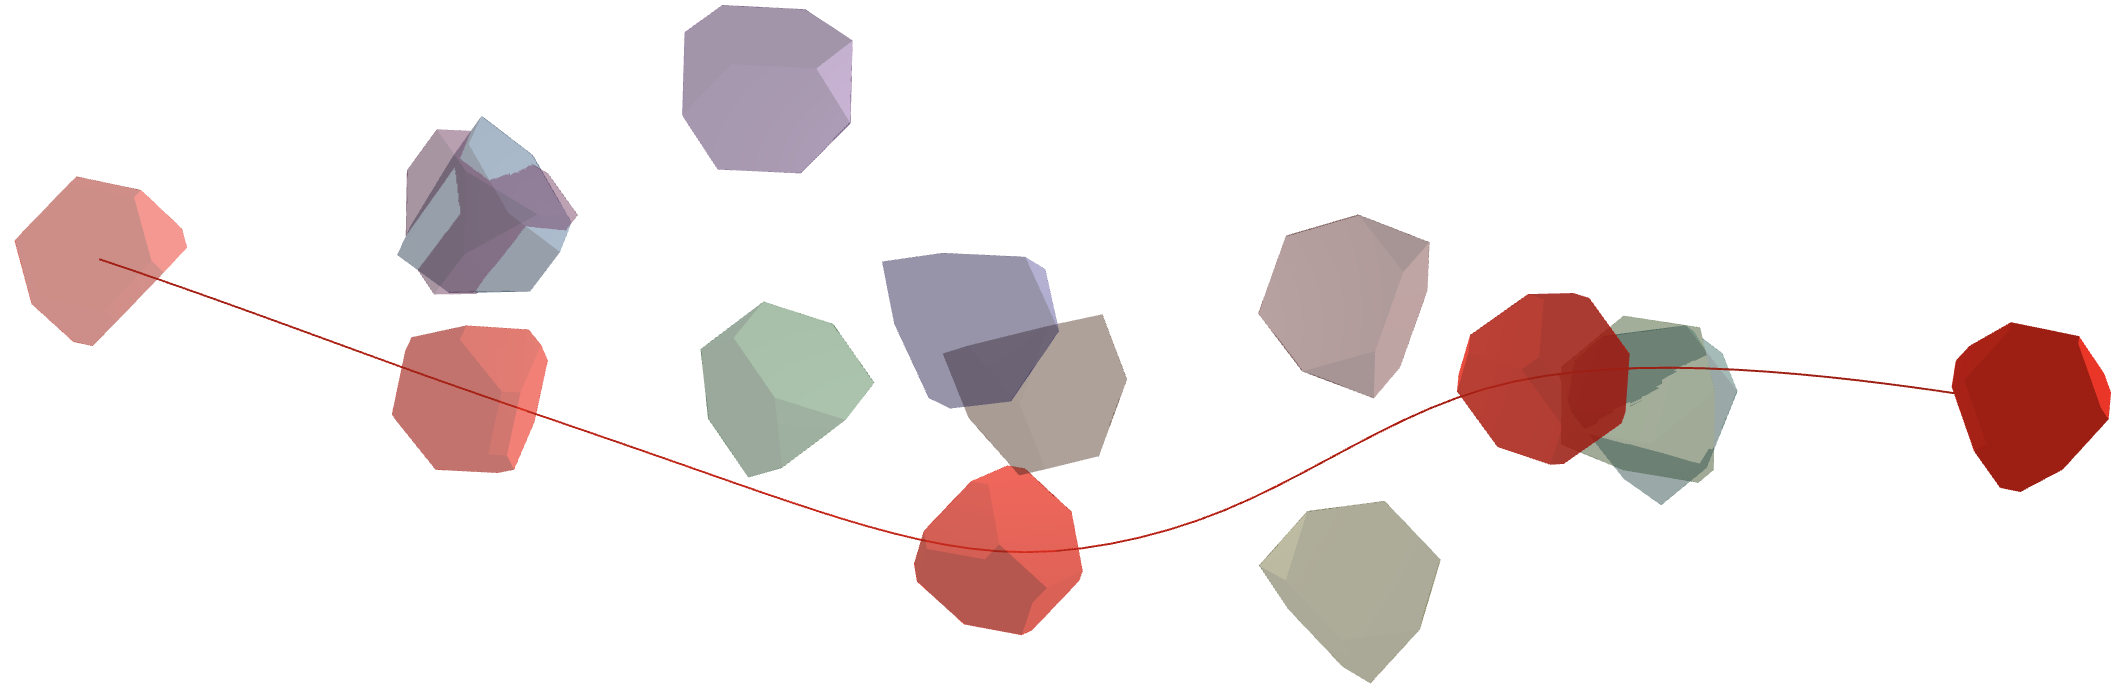
\includegraphics[width=.47\textwidth]{figures/hallway/hallway1.png}
    \caption{A polytope with position and attitude control navigates a field of moving obstacles. Differentiable continuous collision detection is used in a trajectory optimization to solve for the collision-free sequence.}
    \label{fig:hallway2}
\end{figure}


% \begin{figure}
% \centering
% \begin{subfigure}[b]{0.4\textwidth}
%    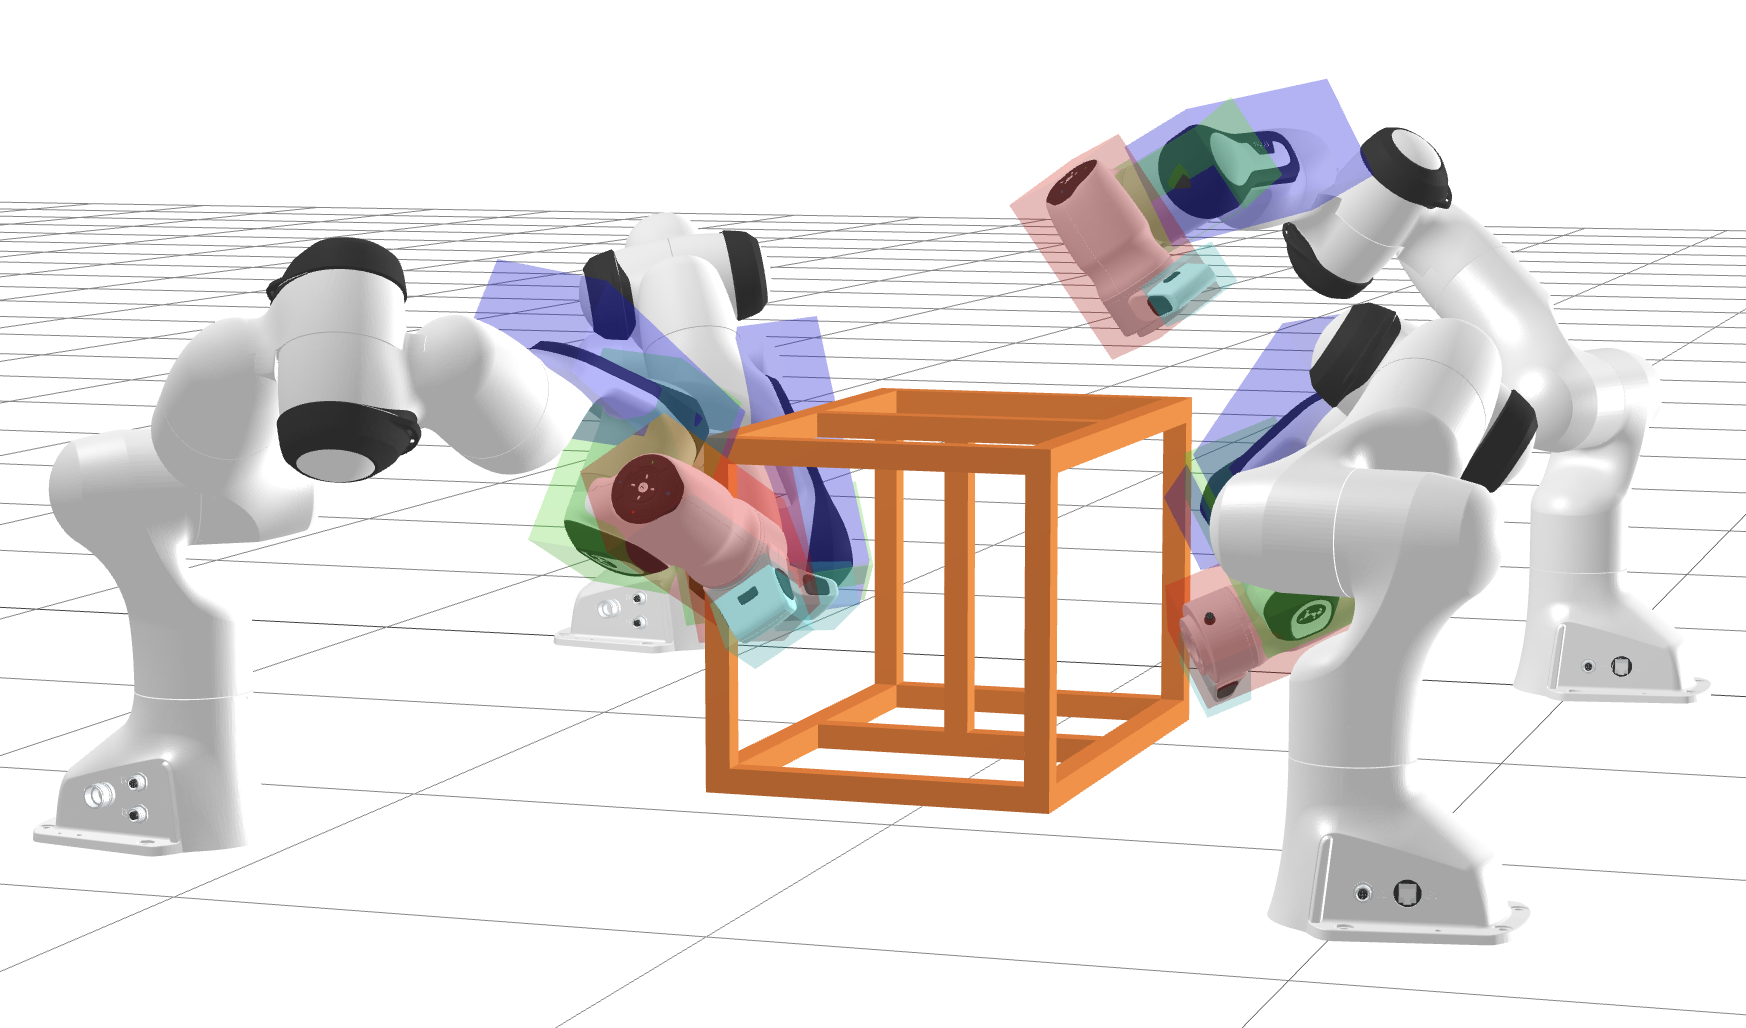
\includegraphics[width=1\linewidth]{figures/ballet/ballet1.png}
%    \caption{}
%    \label{fig:Ng1} 
% \end{subfigure}

% \begin{subfigure}[b]{0.4\textwidth}
%    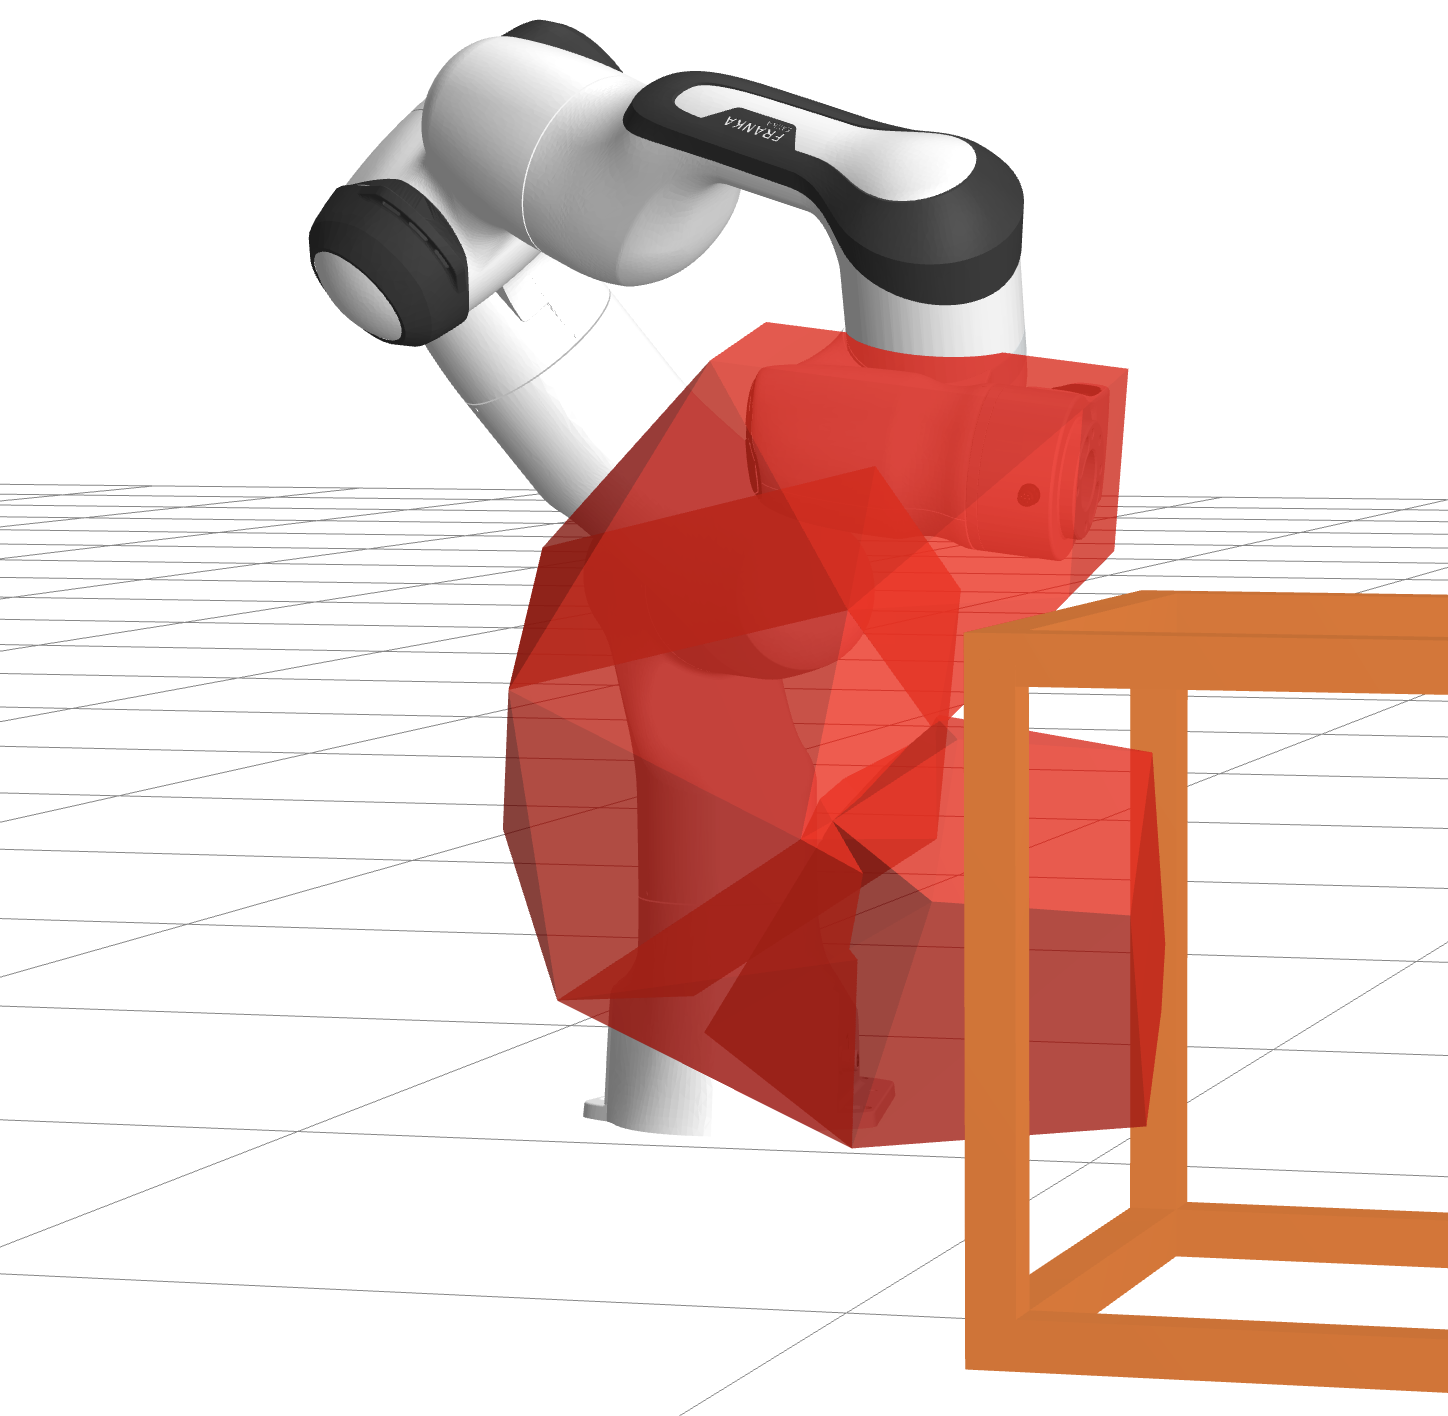
\includegraphics[width=1\linewidth]{figures/ballet/hulls.png}
%    \caption{}
%    \label{fig:Ng2}
% \end{subfigure}

% \caption[Two numerical solutions]{(a) Numerical solutions for the small-time system 
% with a constant-curvature body shape showing the scaled leading-order veritcal 
% reaction force $N_0$ versus the scaled body mass $M$ for various values of $g$. 
% Again, $I=M$ for definiteness and $A=0.7$. (b) As for (a) but over a wider range of 
% values of $M,I$.}
% \end{figure}
% \begin{figure}
% 	\centering
% 	\begin{subfigure}{0.3\linewidth}
% 		\includegraphics[width=\linewidth]{car1.jpg}
% 		\caption{Yellow color}
% 		\label{fig:subfigA}
% 	\end{subfigure}
% 	\begin{subfigure}{0.3\linewidth}
% 		\includegraphics[width=\linewidth]{car2.jpg}
% 		\caption{Red color}
% 		\label{fig:subfigB}
% 	\end{subfigure}
% 	\begin{subfigure}{0.3\linewidth}
% 	        \includegraphics[width=\linewidth]{car3.jpg}
% 	        \caption{Green color}
% 	        \label{fig:subfigC}
%          \end{subfigure}
% 	\caption{Showing three cars in different colors horizontally.}
% 	\label{fig:subfigures}
% \end{figure}


% \begin{figure}
%   \centering
%   \begin{tabular}{@{}c@{}}
%     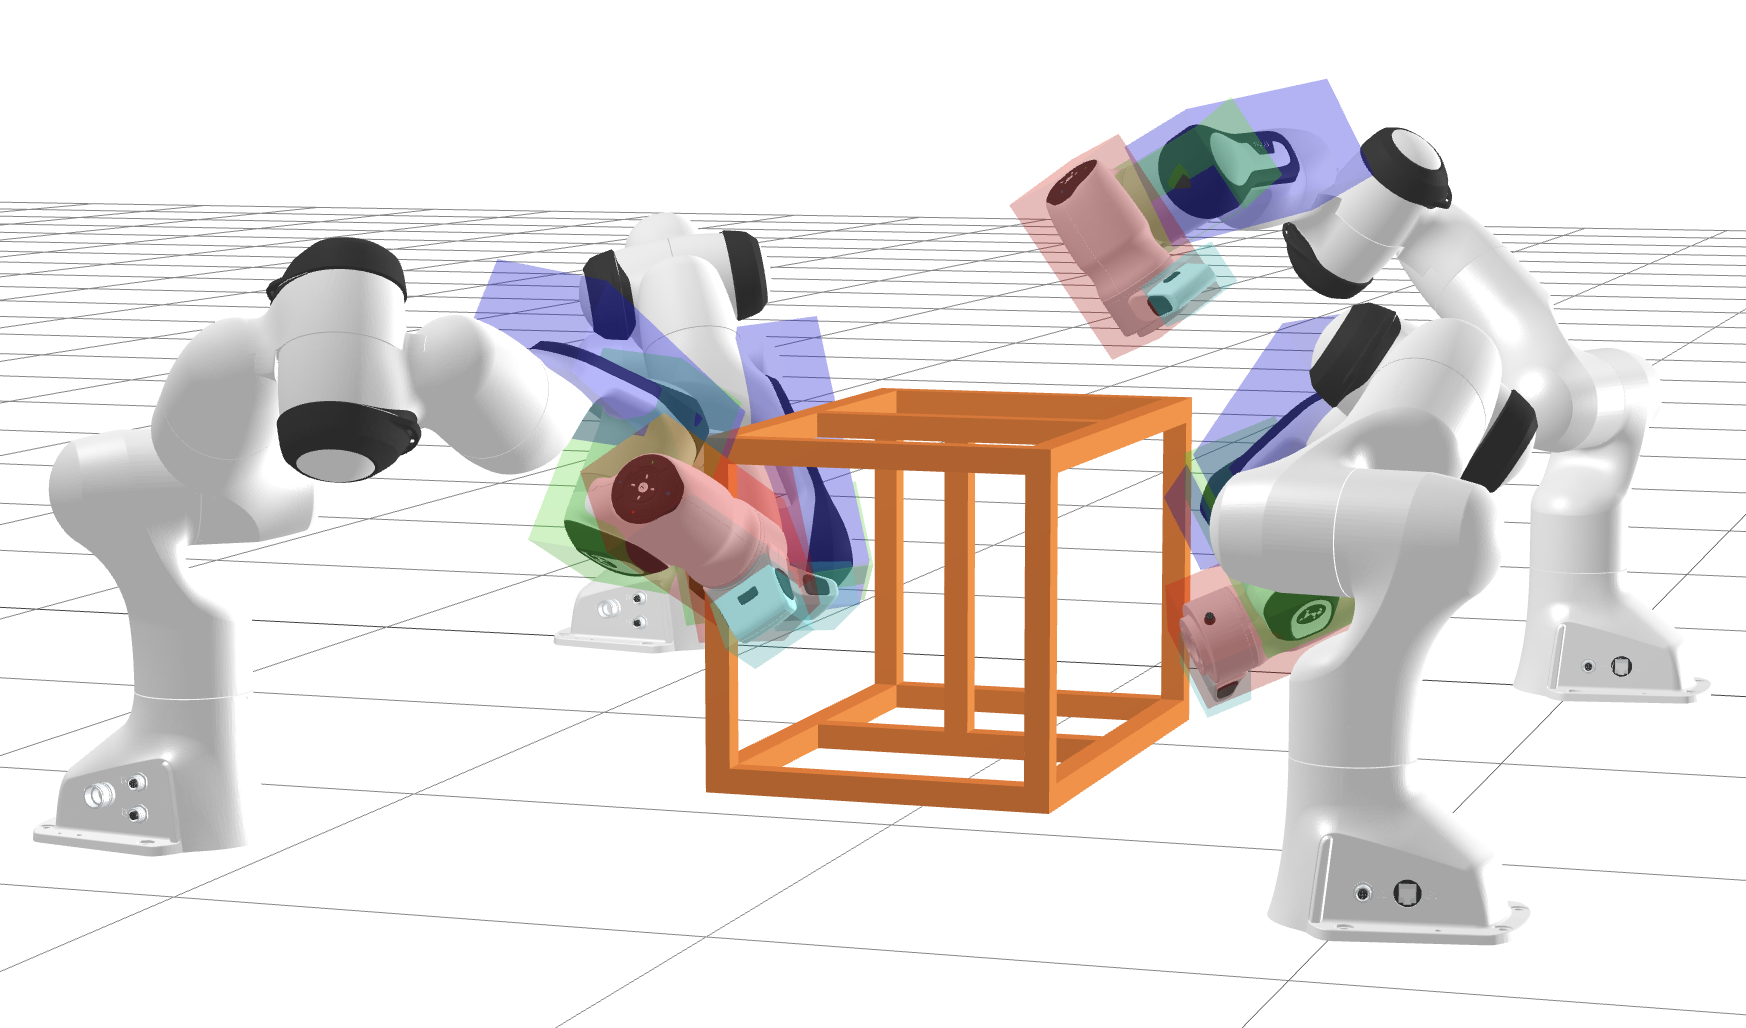
\includegraphics[width=.8\linewidth]{figures/ballet/ballet1.png} \\[\abovecaptionskip]
%     % \small (a) An image
%   \end{tabular}

%   \vspace{\floatsep}

%   \begin{tabular}{@{}c@{}}
%     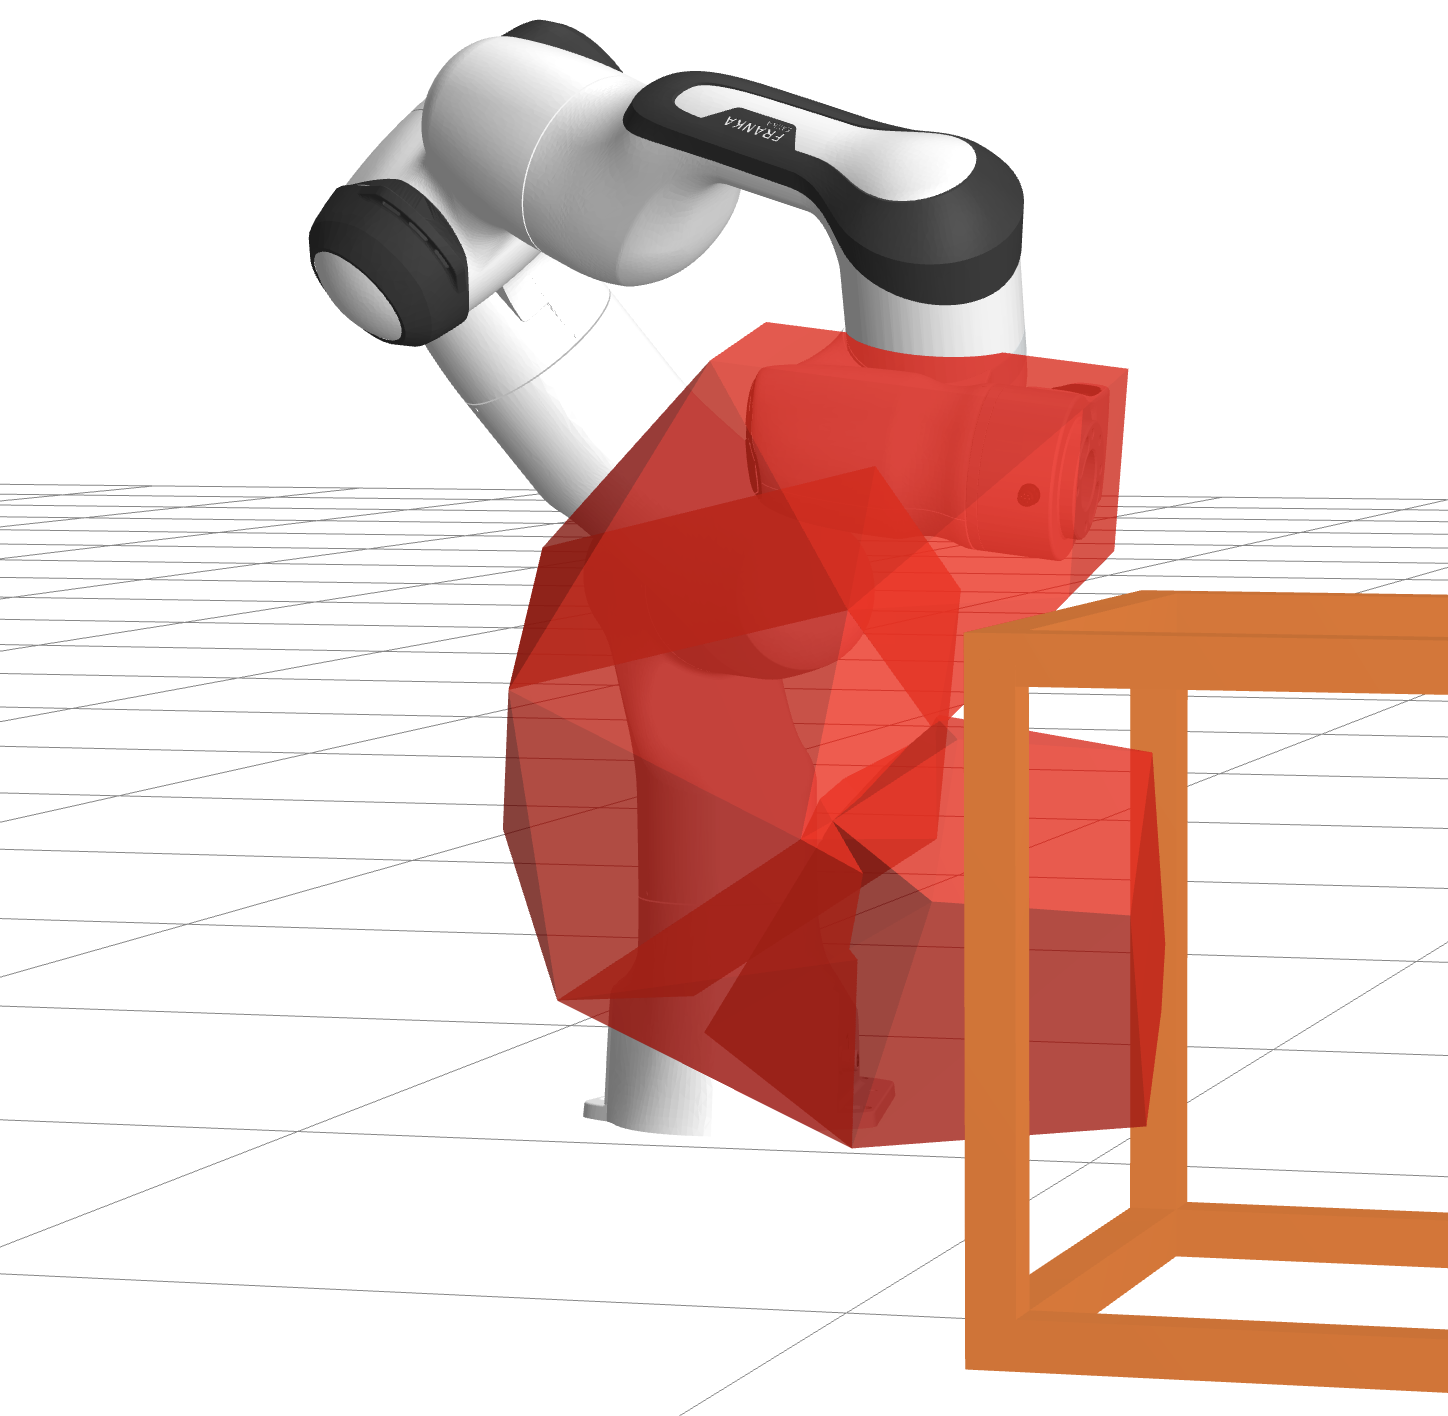
\includegraphics[width=.45\linewidth]{figures/ballet/hulls.png} \\[\abovecaptionskip]
%     % \small (b) Another image
%   \end{tabular}
%   \caption{A multi-robot assembly task where four robotic arms interact with a structure in a common workspace. The proposed continuous collision detection is used to certify collision-free trajectories and is fully differentiable with respect to the configurations of the robots. Shown below is an }\label{fig:ballet}
% \end{figure}


%
%
%
%
The utility of flexible and differentiable CCD is demonstrated in motion-planning examples in which gradient-based trajectory optimization is used to solve for collision-free trajectories. To do this, we consider discrete-time dynamical systems of the form $x_{k+1} = f(x_k, u_k)$, and solve the motion planning problem as a numerical optimization problem:
%
\begin{mini}
{x_{1:N}, u_{1:N-1}}{\sum_{i=1}^{N-1} \ell(x_i, u_i) + \ell_N(x_N)}{\label{trajopt}}{}
\addConstraint{x_1}{= x_{init}}{}
\addConstraint{x_{k+1}}{= f(x_k, u_k)}{\quad i = 1:N-1}
\addConstraint{\alpha(x_k, x_{k+1})}{\geq 1 + d}{\quad i = 1:N-1}
\addConstraint{x_N}{= x_{goal},}{}
\end{mini}
%
where $x_{1:N}$ and $u_{1:N-1}$ are the states and controls for an N-step trajectory, $x_{init}$ and $x_{goal}$ are the initial and final conditions, $\ell(x,u)$ and $\ell_N(x)$ make up the cost function, and $\alpha(x_k, x_{k+1})$ represent the continuous collision constraints that $\alpha$ from \eqref{cdcol} must be greater than $1 + d$, where $d \in \mathbb{R}_+$ is some margin. From here, this problem can be solved with generic nonlinear programming (NLP) solvers like SNOPT \cite{gill2005} or Ipopt \cite{wachter2006}.
%
%
\subsection{Tunneling}
%
%
The first example, shown in Fig. \ref{fig:thru_wall}, showcases a classic failure mode of discrete collision checking --- tunneling. Trajectory optimization is used to find a trajectory that guides a polytope around a wall, and we directly compare the optimal trajectories when DCD and CCD are used. With DCD (shown in red), the polytope passes directly through the wall in a straight line towards the goal. On inspection, this is clearly an infeasible trajectory despite each the configuration at each time step being out of collision. Since the solver can only reason about discrete collision checks, it is a feasible and optimal trajectory in the context of the solver. With our differentiable CCD, even with a very coarse trajectory discretization, the solver is able to avoid tunneling and navigate around the wall instead of through it. 
% \todo{trim this section}
%
%
\subsection{Moving Obstacles}
%
%
In this example, shown in Fig. \ref{fig:hallway2}, trajectory optimization with CCD constraints is used to navigate a polytope through a field of moving obstacles. Every object in this scene is moving, and the CCD is able to reason directly about this motion to ensure that there are no accidental collisions.  The resulting collision-free trajectory successfully takes the polytope from the start to the goal without hitting any of the ten obstacles.
%
%
\subsection{Multi-Robot Assembly}
\begin{figure}[t!]
    \centering
    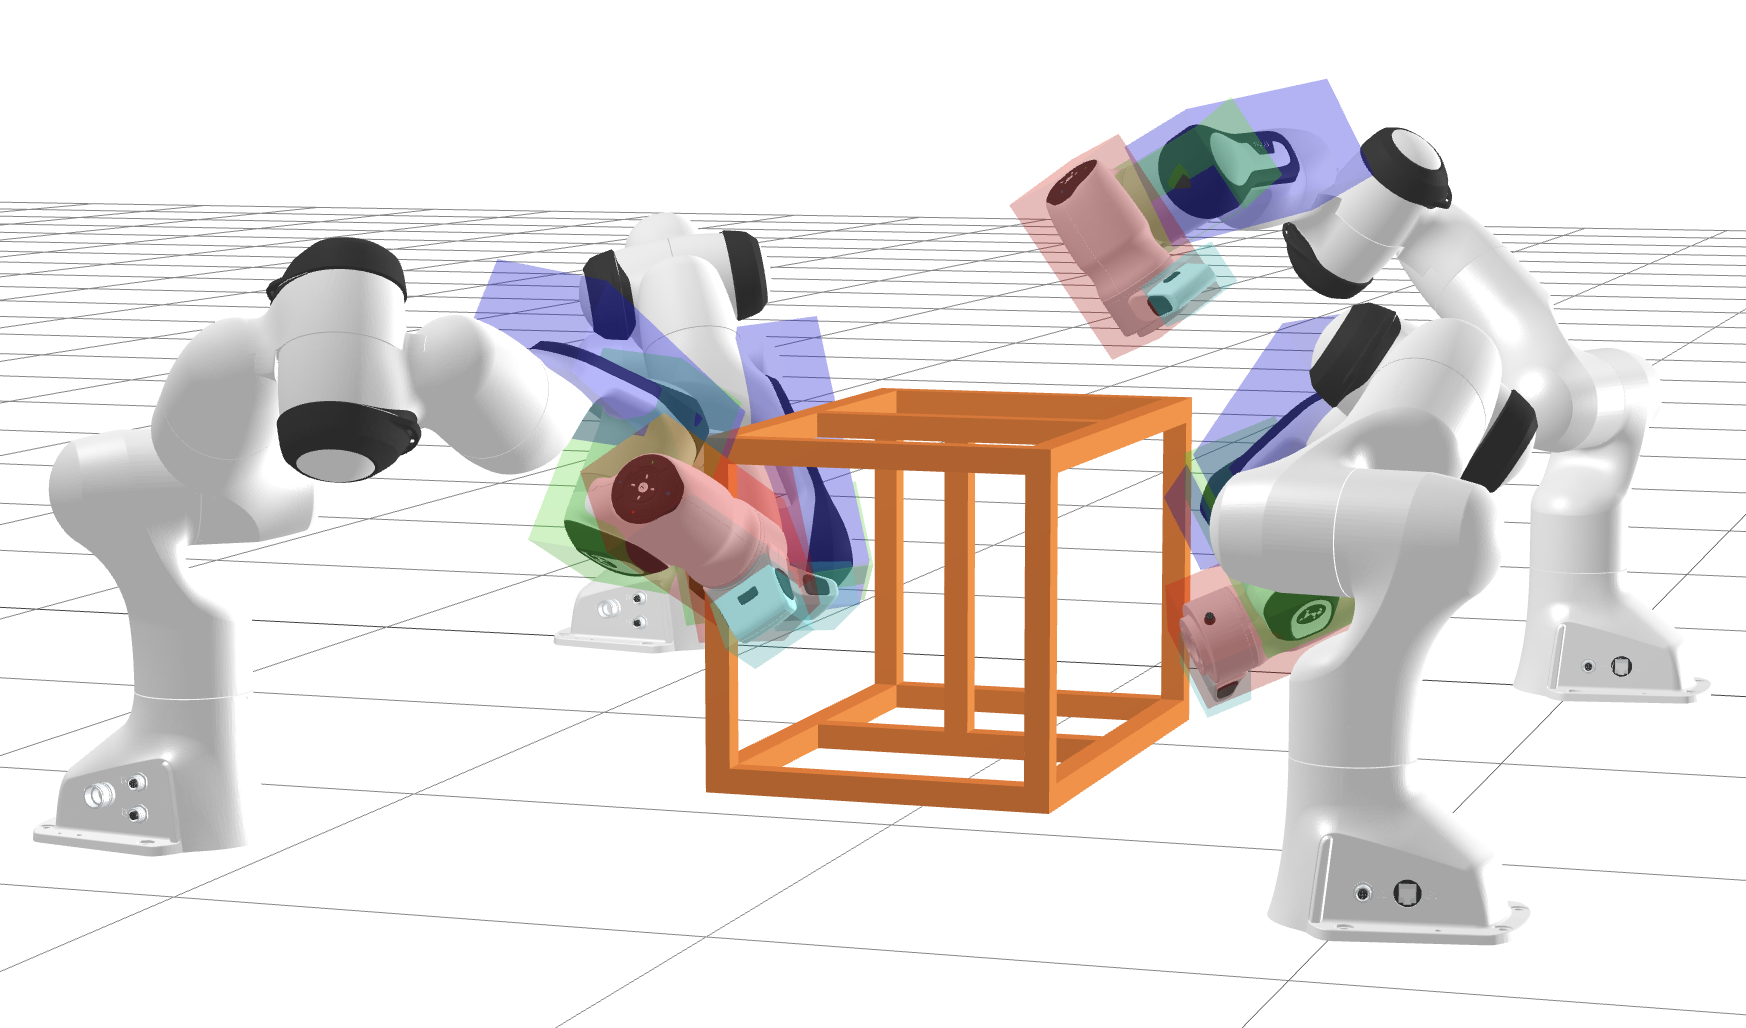
\includegraphics[width=.47\textwidth]{figures/ballet/ballet1.png}
    \caption{A multi-robot assembly task where four robotic arms interact with a structure in a common workspace. The proposed continuous collision detection is used to certify collision-free trajectories and is fully differentiable with respect to the configurations of the robots.}
    \label{fig:ballet}
\end{figure}
As shown in Fig. \ref{fig:ballet}, this scenario involes four Franka Panda robots completing a mock assembly task in unison in a shared workspace. The robots have had their end effectors discretized into convex sets and are interacting with a structure made up of polytopes. CCD ensures the whole operation is collision-free, even between timesteps.
% \todo{I can't get the multi-franka example working so I have to settle for a nother arm example}
% \subsection{Multi-Robot Manipulation}
% %
% %
% As shown in Fig. \todo{make fig}, this example uses differentiable continuous collision checking to ensure that four Franka Panda robots do not collide with each other or the obstacles in the workspace during a group manipulation task. By decomposing both the environment and robots into polytopes, the proposed continuous collision framework is used to generate differentiable collision constraints used by the trajectory optimization solver. This guarantees that the end effectors of the robots will not tunnel through the environment or eachother, avoiding any accidental collisions. 
% %
% %
% %
% %
\section{Conclusion}\label{sec:cdcol:conclusion}
%
%
%
%
In this paper we present a fully differentiable continuous collision-detection framework that is fast, robust, and entirely branch free. This algorithm is readily parallelized in modern compute frameworks such as JAX, and directly integrates with automatic differentiation tools for seamless differentiation through the routine. The resulting method is used in gradient-based trajectory optimization problems as collision avoidance constraints and is demonstrated on a range of practical examples.  

%%% Local Variables:
%%% coding: utf-8
%%% mode: latex
%%% TeX-engine: xetex
%%% TeX-master: "../thesis"
%%% End: